%Version 3.1 December 2024
% See section 11 of the User Manual for version history
%
%%%%%%%%%%%%%%%%%%%%%%%%%%%%%%%%%%%%%%%%%%%%%%%%%%%%%%%%%%%%%%%%%%%%%%
%%                                                                 %%
%% Please do not use \input{...} to include other tex files.       %%
%% Submit your LaTeX manuscript as one .tex document.              %%
%%                                                                 %%
%% All additional figures and files should be attached             %%
%% separately and not embedded in the \TeX\ document itself.       %%
%%                                                                 %%
%%%%%%%%%%%%%%%%%%%%%%%%%%%%%%%%%%%%%%%%%%%%%%%%%%%%%%%%%%%%%%%%%%%%%

%%\documentclass[referee,sn-basic]{sn-jnl}% referee option is meant for double line spacing

%%=======================================================%%
%% to print line numbers in the margin use lineno option %%
%%=======================================================%%

%%\documentclass[lineno,pdflatex,sn-basic]{sn-jnl}% Basic Springer Nature Reference Style/Chemistry Reference Style

%%=========================================================================================%%
%% the documentclass is set to pdflatex as default. You can delete it if not appropriate.  %%
%%=========================================================================================%%

%%\documentclass[sn-basic]{sn-jnl}% Basic Springer Nature Reference Style/Chemistry Reference Style

%%Note: the following reference styles support Namedate and Numbered referencing. By default the style follows the most common style. To switch between the options you can add or remove �Numbered� in the optional parenthesis. 
%%The option is available for: sn-basic.bst, sn-chicago.bst%  
 
%%\documentclass[pdflatex,sn-nature]{sn-jnl}% Style for submissions to Nature Portfolio journals
%%\documentclass[pdflatex,sn-basic]{sn-jnl}% Basic Springer Nature Reference Style/Chemistry Reference Style
%%\documentclass[pdflatex,sn-mathphys-num]{sn-jnl}% Math and Physical Sciences Numbered Reference Style
%%\documentclass[pdflatex,sn-mathphys-ay]{sn-jnl}% Math and Physical Sciences Author Year Reference Style
%%\documentclass[pdflatex,sn-aps]{sn-jnl}% American Physical Society (APS) Reference Style
\documentclass[pdflatex,sn-vancouver-num]{sn-jnl}% Vancouver Numbered Reference Style
%%\documentclass[pdflatex,sn-vancouver-ay]{sn-jnl}% Vancouver Author Year Reference Style
%%\documentclass[pdflatex,sn-apa]{sn-jnl}% APA Reference Style
%%\documentclass[pdflatex,sn-chicago]{sn-jnl}% Chicago-based Humanities Reference Style

%%%% Standard Packages
%%<additional latex packages if required can be included here>

\usepackage[T1]{fontenc}
\usepackage{graphicx}%
\usepackage{multirow}%
\usepackage{amsmath,amssymb,amsfonts}%
\usepackage{amsthm}%
\usepackage{mathrsfs}%
\usepackage[title]{appendix}%
\usepackage{xcolor}%
\usepackage{textcomp}%
\usepackage{manyfoot}%
\usepackage{booktabs}%
\usepackage{algorithm}%
\usepackage{algorithmicx}%
\usepackage{algpseudocode}%
\usepackage{listings}%
\usepackage{enumitem}
\usepackage{subcaption}
\usepackage{microtype}
\usepackage{natbib}
\usepackage{bibunits}
\usepackage{array}
\setlength{\emergencystretch}{2em}
%%%%


%% as per the requirement new theorem styles can be included as shown below
\theoremstyle{thmstyleone}%
\newtheorem{theorem}{Theorem}%  meant for continuous numbers
%%\newtheorem{theorem}{Theorem}[section]% meant for sectionwise numbers
%% optional argument [theorem] produces theorem numbering sequence instead of independent numbers for Proposition
\newtheorem{proposition}[theorem]{Proposition}% 
%%\newtheorem{proposition}{Proposition}% to get separate numbers for theorem and proposition etc.

\theoremstyle{thmstyletwo}%
\newtheorem{example}{Example}%
\newtheorem{remark}{Remark}%

\theoremstyle{thmstylethree}%
\newtheorem{definition}{Definition}%

\raggedbottom
%%\unnumbered% uncomment this for unnumbered level heads

\begin{document}

\title[Article Title]{TaxaLoom: interactive exploration of sample-level taxonomic abundance profiles in microbiome datasets}

%%=============================================================%%
%% GivenName	-> \fnm{Joergen W.}
%% Particle	-> \spfx{van der} -> surname prefix
%% FamilyName	-> \sur{Ploeg}
%% Suffix	-> \sfx{IV}
%% \author*[1,2]{\fnm{Joergen W.} \spfx{van der} \sur{Ploeg} 
%%  \sfx{IV}}\email{iauthor@gmail.com}
%%=============================================================%%

\author[1,2]{\fnm{Antonin} \sur{Colajanni}}\email{antonin.colajanni@u-bordeaux.fr}

\author[2]{\fnm{Frederic} \sur{Lalanne}}\email{frederic.lalanne@u-bordeaux.fr}


\author[]{\fnm{Jef} \sur{Ceulemans}}%\email{jef.ceulemans@proximus.be}
\equalcont{These authors contributed equally to this work.}

\author[]{\fnm{Stijn} \spfx{De} \sur{Busser}}%\email{stain.debusser@gmail.com}
\equalcont{These authors contributed equally to this work.}

\author[1,3,4]{\fnm{Rodolphe} \sur{Thiébaut}}\email{rodolphe.thiebaut@u-bordeaux.fr}

\author[2]{\fnm{Romain} \sur{Bourqui}}\email{romain.bourqui@labri.fr}

\author*[2]{\fnm{Patricia} \sur{Thébault}}\email{patricia.thebault@u-bordeaux.fr}




\affil*[1]{
    \orgdiv{Université de Bordeaux}, 
    \orgname{INSERM, Inria, BPH, U1219}, 
    \orgaddress{\street{146 rue Léo Saignat 11}, \city{Bordeaux}, 
    \postcode{33076}, \country{France}}}

\affil[2]{
    \orgdiv{LaBRI}, 
    \orgname{UMR CNRS 5800}, 
    \orgaddress{
        \street{351 cours de la libération}, \city{Talence}, \postcode{33405}, \country{France}}}

\affil*[3]{
    \orgdiv{CHU de Bordeaux, Service d'information Médicale}, 
    \orgname{INSERM U1219}, 
    \orgaddress{\city{Bordeaux}, \country{France}}}

\affil*[4]{
    \orgdiv{Vaccine Research Institute}, 
    \orgname{Université Paris-Est Créteil, Faculté de Médecine, INSERM U955}, 
    \orgaddress{\street{51 Av Marechal de Lattre de Tassigny}, \city{Créteil}, \postcode{94010}, \country{France}}}



\abstract{


\textbf{Background:}
High-throughput sequencing technologies generate microbial taxonomic abundance profiles across large numbers of samples and taxa. Exploring these data remains challenging due to the hierarchical structure of microbial taxonomy and characteristics such as differences in sequencing depth, sparsity, compositionality, and highly skewed abundance distributions. These properties complicate comparisons between samples and make it difficult to identify patterns from abundance values alone. Different normalization and transformation methods have been implemented to account for these characteristics, but their application can influence the resulting abundance profiles. In parallel, biological, clinical, and technical metadata need to be considered when investigating microbial abundance patterns. As the number of taxa and samples increases, these relationships become difficult to examine using abundance tables or summary statistics alone. Interactive visualization provides a complementary approach by allowing users to explore taxonomic profiles, examine individual samples and their associated metadata, and compare the effects of different preprocessing strategies.


\textbf{Results:}
We present TaxaLoom, a web-based application for the interactive exploration of microbial taxonomic abundance profiles. TaxaLoom combines an interactive taxonomic tree with synchronized parallel coordinates and swarm plots, which display individual sample abundances as separate points, to examine abundance distributions across samples. The application integrates sample metadata visualization, interactive filtering, and multiple normalization and transformation methods, allowing users to explore and compare individual samples while considering different preprocessing strategies. Two case applications illustrate these capabilities. In an HIV cohort, TaxaLoom was used to compare preprocessing methods and to explore microbial abundance patterns in relation to both categorical and quantitative clinical metadata, including immune response status and CD4 T-cell counts. In TCGA data, progressive exploration of the taxonomic hierarchy allowed taxa with distinct abundance patterns to be identified, while comparison with technical metadata revealed associations with sequencing centre and read length that were consistent with potential technical artefacts or contamination.

\textbf{Conclusions:}
TaxaLoom facilitates the exploration of microbial abundance profiles by integrating taxonomic navigation, sample-level visualization, metadata, and preprocessing within a common interface, providing a new original approach to existing microbiome analysis workflows.


}


\keywords{Microbiome; Taxonomic abundance; Interactive visualization; Exploratory data analysis; Data normalization}

\maketitle


\section{Background}\label{sec1}

High-throughput sequencing has enabled the characterization of complex microbial communities across biological, clinical, and environmental contexts. Taxonomic profiling commonly relies on marker-gene amplicon sequencing or shotgun metagenomics \cite{jovel_characterization_2016,durazzi_comparison_2021}. Marker-gene approaches target taxonomically informative regions, most commonly the 16S rRNA gene for bacterial and archaeal communities, to identify operational taxonomic units (OTUs). In contrast, shotgun metagenomics sequences DNA without targeting specific genomic regions, enabling broader taxonomic and functional characterization \cite{jovel_characterization_2016,durazzi_comparison_2021,breitwieser_review_2019}. Metatranscriptomic sequencing similarly profiles microbial communities from RNA, providing information on transcriptionally active microorganisms and their expressed functions \cite{breitwieser_review_2019,bashiardes_use_2016}. Despite their methodological differences, these approaches can generate taxonomic abundance profiles describing the microorganisms detected across multiple samples.

The interpretation of microbial abundance profiles depends not only on taxonomic abundances but also on information associated with the samples themselves. Large-scale initiatives such as the Human Microbiome Project (HMP) have contributed to characterizing the human microbiome and its variability across individuals and body sites \citep{huttenhower_structure_2012,proctor_integrative_2019}. Beyond characterizing microbial communities, combining microbial abundance profiles with biological and clinical metadata allows researchers to investigate their associations with specific phenotypes. For example, differences in gut microbial composition have been associated with type 2 diabetes \citep{qin_metagenome-wide_2012}, while other studies have investigated associations between gut microbial profiles and response to cancer immunotherapy \citep{routy_gut_2018,gopalakrishnan_gut_2018}.

However, not all variations in microbial abundance profiles necessarily reflect differences associated with the phenotype of interest. Biological factors, such as diet, environmental conditions, or host genetics, can influence microbial composition and potentially confound associations with clinical outcomes \citep{huttenhower_structure_2012}. Furthermore, technical factors associated with sample collection, processing, library preparation, or sequencing can introduce systematic differences between samples. For example, microbial contaminants can vary between laboratories, reagents, and reagent batches \citep{salter_reagent_2014,laurence_common_2014}. Cross-sample contamination represents another potential source of technical bias, as microbial sequences originating from one sample may be incorrectly attributed to another \citep{goulet_crocodeel_2026}. Consequently, both biological and technical metadata, are important for investigating potential sources of variation in microbial abundance profiles.


Beyond these limitations, microbial sequencing data also present challenges associated with their compositional nature. When expressed as proportions, the abundance of each taxon is interpreted relative to the other taxa in the sample rather than independently. These proportions are constrained to sum to one, meaning that changes in the relative abundance of one taxon can affect the proportions of others \citep{quinn_understanding_2018,aitchison_statistical_1982}. Alongside compositionality, microbial abundance data also tend to be highly sparse, with a large proportion of zero values. However, these zeros can have different origins: they may indicate the true absence of a taxon from a sample, or result from limited sequencing depth that prevents the detection of low-abundance microorganisms \citep{chan_zero_2024}. Furthermore, microbial count data frequently exhibit overdispersion, with variability exceeding that expected under a Poisson distribution \citep{lin_analysis_2020}. These characteristics complicate statistical analyses and the comparison of microbial abundance profiles across samples.

Numerous preprocessing strategies have been proposed to address the characteristics of microbial abundance data. Here, normalization refers to methods that make abundance values more comparable across samples, whereas transformation refers to changes in the mathematical scale on which values are represented. These operations are not mutually exclusive, and many preprocessing strategies combine both. The term \textit{preprocessing strategies} will therefore be used hereafter to encompass normalization, transformation, and approaches that draw from both. Some normalization methods primarily account for differences in sequencing depth by adjusting read counts using sample-specific scaling factors \citep{weiss_normalization_2017}. Other approaches address the compositional nature of the data through log-ratio transformations, which analyse taxa relative to one another rather than as independent abundances \citep{quinn_understanding_2018}. Sparsity also requires particular consideration, as some normalization methods explicitly account for the large number of zeros in microbial abundance data \citep{chen_gmpr_2018,martino_novel_2019}. Finally, transformations such as logarithmic or square root transformations can reduce the large differences between observed abundance values, although logarithmic transformations require special treatment of zero counts.


%Importantly, these approaches rely on different assumptions and may preserve or emphasize different characteristics of the same dataset. Benchmarking studies have demonstrated that preprocessing choices can influence downstream analyses, including differential abundance testing \citep{weiss_normalization_2017,nearing_microbiome_2022}, taxon-metadata associations \citep{llorens-rico_benchmarking_2021}, and phenotype prediction \citep{wang_comparison_2024}. Their relative performance therefore depends not only on the characteristics of the dataset but also on the objectives of the analysis, with no single strategy being optimal in every setting. In an exploratory context, visualizing abundance profiles under different preprocessing strategies can provide complementary views of the same dataset. Comparing these representations allows researchers to examine how preprocessing choices influence the observed patterns and whether these patterns remain consistent across methods.

Importantly, these approaches rely on different assumptions and may preserve or emphasize different characteristics of the same dataset. Benchmarking studies have demonstrated that preprocessing choices can influence downstream analyses, including differential abundance testing \citep{weiss_normalization_2017,nearing_microbiome_2022}, taxon-metadata associations \citep{llorens-rico_benchmarking_2021}, phenotype prediction \citep{wang_comparison_2024}, and the selection of microbial features in predictive models \citep{karwowska_effects_2025}. Different preprocessing strategies may also involve trade-offs between analytical performance and biological interpretation. For example, some transformations can produce comparable phenotype classification performance while identifying substantially different microbial features as important predictors \citep{karwowska_effects_2025}. Their relative performance therefore depends not only on the characteristics of the dataset but also on the objectives of the analysis, with no single strategy being optimal in every setting. In an exploratory context, visualizing abundance profiles under different preprocessing strategies can provide complementary views of the same dataset. Comparing these representations allows researchers to examine how preprocessing choices influence the observed patterns and whether these patterns remain consistent across methods.

Beyond preprocessing considerations, the interpretation of microbial abundance profiles also requires examining individual observations. As famously illustrated by Anscombe's quartet \citep{anscombe_graphs_1973}, datasets with similar descriptive statistics can exhibit very different patterns when visualized.

In microbiome research, several questions can arise during this exploration: how does the abundance of a particular taxon vary across samples? Are the observed patterns associated with biological or clinical characteristics, or with technical factors? At which taxonomic level does a separation between metadata-defined groups become apparent? Do these patterns persist when different preprocessing strategies are applied? Addressing these questions requires navigating the taxonomic hierarchy, comparing individual sample abundances, integrating sample metadata, and examining the same abundance profiles under different preprocessing strategies. Interactive visualization can support these tasks by allowing researchers to progressively explore the data and investigate relationships between these different dimensions.

Several tools have been developed to support different aspects of microbiome data exploration (Table~\ref{tab:tool_comparison}). These tools rely on different visual metaphors, sometimes shared across applications, to represent taxonomic hierarchies, microbial abundances, and relationships between samples. Each representation offers different possibilities for exploring the data, depending on the information being examined and the analytical task. Krona uses an interactive sunburst chart to navigate hierarchical taxonomic profiles \citep{ondov_interactive_2011}, Metacoder represents taxonomic abundances and differences between groups using heat trees \citep{foster_metacoder_2017}, and Pavian uses Sankey diagrams to represent the distribution of reads across taxonomic levels, complemented by heatmaps for multi-sample comparisons \citep{breitwieser_pavian_2020}. Other tools integrate multiple visualization techniques within broader microbiome analysis environments. Shiny-phyloseq provides bar plots, heatmaps, phylogenetic trees, ordination plots, and interactive network representations \citep{mcmurdie_shiny-phyloseq_2015}. QIIME2 View provides browser-based exploration of QIIME 2 outputs through interactive visualizations including taxonomic bar plots at different taxonomic levels, PCoA ordination plots, alpha-diversity raincloud plots, and summary statistics \citep{bolyen_reproducible_2019}. MicrobiomeAnalyst combines statistical and preprocessing methods with interactive stacked bar plots, heatmaps, and other representations for microbiome data exploration \citep{lu_microbiomeanalyst_2023}. Metaviz combines its FacetZoom representation for navigating the taxonomic hierarchy with coordinated heatmaps, stacked bar plots, and other sample-level visualizations, allowing users to interactively select and highlight corresponding data across multiple views \citep{wagner_metaviz_2018}. Snowflake represents microbiome data as bipartite graphs connecting sample nodes to the microbial features detected within them, allowing the identification of shared microorganisms while incorporating taxonomic annotations and sample metadata \citep{peeters_snowflake_2024}.

While these tools provide complementary approaches to microbiome visualization, they differ in the functionalities available for exploring taxonomic hierarchies, individual samples, associated metadata, and preprocessing choices. In particular, the integration of these different aspects within a single interactive environment remains limited, especially regarding the direct comparison of normalization methods.

Here, we present TaxaLoom, a web-based application designed to address the challenges of jointly exploring microbial abundance patterns, taxonomic relationships, and associated sample metadata.TaxaLoom combines an interactive taxonomic tree with synchronized parallel coordinates and swarm plots, where individual samples are represented as lines across multiple taxa and as points showing their abundance distributions, respectively. Together, these representations allow users to examine overall abundance patterns while following individual samples across different taxa. The application also integrates biological and technical metadata to investigate associations with microbial abundances, alongside multiple preprocessing strategies to examine how different normalization and transformation methods influence observed patterns. Although developed using shotgun RNA-sequencing data, TaxaLoom can be applied to taxonomic abundance profiles provided as raw count data, independently of the sequencing approach used to generate them.





\newcommand{\fixedrow}{\rule[-0.45cm]{0pt}{0.8cm}}

\begin{sidewaystableorg}[p]
\centering
\caption{\textbf{Comparison of TaxaLoom with existing tools for the visualization and exploration of microbiome taxonomic abundance data.} Features refer to functionalities described in the corresponding publications.}
\label{tab:tool_comparison}
%\normalsize
\resizebox{\linewidth}{!}{%
\setlength{\tabcolsep}{3pt}
\renewcommand{\arraystretch}{1.5}
\setlength{\extrarowheight}{8pt}
\begin{tabular}{>{\raggedright\arraybackslash}m{3.5cm}ccccccccc}
\hline
\textbf{Feature}
& \textbf{TaxaLoom}
& \textbf{QIIME2 view \cite{bolyen_reproducible_2019}}
& \textbf{Pavian \cite{breitwieser_pavian_2020}}
& \textbf{Metacoder \cite{foster_metacoder_2017}}
& \textbf{MicrobiomeAnalyst \cite{lu_microbiomeanalyst_2023}}
& \textbf{Shiny-phyloseq \cite{mcmurdie_shiny-phyloseq_2015}}
& \textbf{Krona \cite{ondov_interactive_2011}}
& \textbf{Metaviz \cite{wagner_metaviz_2018}}
& \textbf{Snowflake \cite{peeters_snowflake_2024}} \\
\hline
 Interface/access mode
& Web application
& Web application
& R/Shiny; web application
& R package
& Web application
& R/Shiny
& Browser-based
& Web application + R session
& R package \\
 Input type
& Tabular
& QIIME2 output
& Tabular
& Tabular
& BIOM; tabular
& BIOM
& Tabular
& Tabular
& Tabular \\
 Interactive visualization
& Yes & Yes & Yes & No & Yes & Yes & Yes & Yes & Yes \\
 Taxonomic hierarchy visualization
& Yes & Yes & Yes & Yes & Yes & Yes & Yes & Yes & Limited \\
 Interactive taxonomic filtering
& Yes & No & Yes & No & No & No & Limited & Yes & No \\
 Simultaneous visualization of multiple samples
& Yes & Yes & Yes & Yes & Yes & Yes & No & Yes & Yes \\
 Sample metadata integration
& Yes & Limited & No & Yes & Yes & Yes & No & Yes & Yes \\
 Synchronized interactive views
& Yes & No & No & No & No & No & No & Yes & Yes \\
 Built-in normalization
& Yes & No & No & Yes & Yes & No & No & No & No \\
 Integrated comparison of normalization methods
& Yes & No & No & No & No & No & No & No & No \\
\hline
\end{tabular}
}
\begin{flushleft}
\footnotesize Yes, functionality available; No, functionality not identified in the corresponding publication or online tool; Limited, functionality available only for a restricted subset of the described feature.
\end{flushleft}
\end{sidewaystableorg}


\section{Implementation}\label{sec2}

\subsection{Technical implementation}

TaxaLoom is a web-based application developed using the Angular framework, with TypeScript as its primary programming language, alongside HTML and CSS for the user interface. As a browser-based application, TaxaLoom is platform-independent and can be accessed through modern desktop web browsers, including Firefox, Chromium, Google Chrome, Microsoft Edge, and GNOME Web. Compatibility with mobile browsers has not been evaluated.

The application can be built and run locally using Node Package Manager (npm) and Angular CLI, tested with versions 11.19.0 and 21, respectively. TaxaLoom is distributed under the MIT license, allowing its use, modification, and redistribution without restrictions specific to academic or non-academic users.

\subsection{TaxaLoom workflow and input data}

TaxaLoom is designed for the interactive exploration of taxonomic abundance profiles together with sample-associated metadata. The application requires an abundance matrix containing taxon abundances across samples, the corresponding taxonomic information, and sample metadata. Taxonomic information provides the hierarchical relationships between detected taxa, whereas metadata can include categorical or quantitative variables describing biological, clinical, or technical characteristics of the samples. Although the Biological Observation Matrix (BIOM) format supports both abundance data and metadata \citep{mcdonald_biological_2012}, TaxaLoom currently uses separate input tables to facilitate the identification and selection of metadata variables during interactive exploration.

The workflow combines these data into linked representations of the taxonomic structure, sample-level abundance profiles, and sample metadata. Users can navigate between taxonomic levels, restrict the visualization to selected taxa or samples, compare abundance profiles according to metadata variables, and apply different normalization or transformation methods. The data corresponding to the current selection can subsequently be displayed in tabular form and exported for further analysis.


\subsection{Interactive visualization}
% taxonomic tree
% parallel coordinates
% swarm plots
% linked views
% selection/filtering
% categorical and quantitative metadata



Taxonomic data are inherently hierarchical, and exploring different taxonomic levels is essential for interpreting microbial abundance profiles. For example, differences between groups of samples may be apparent at a particular taxonomic level but remain hidden at broader or finer resolutions. TaxaLoom therefore represents this hierarchy as an interactive tree, allowing users to navigate between taxonomic levels and select taxa of interest through search and filtering options. This follows Shneiderman's ``overview first, zoom and filter, then details-on-demand'' principle \citep{shneiderman_eyes_1996}.

Parallel coordinates were selected to preserve the identity of individual samples while comparing their abundances across multiple taxa. By representing each sample as a line connecting its abundance values across taxon-specific axes, this representation makes it possible to follow sample-level profiles and identify samples showing similar patterns across taxa. Swarm plots provide a complementary view by displaying the distribution of individual abundance values for each taxon. Linking the two representations combines these advantages: a sample highlighted in one view is simultaneously identified in the other, allowing its position within a taxon-specific distribution to be related to its broader abundance profile. Both representations support linear and logarithmic scales.

%Taxonomic abundances are simultaneously displayed using parallel coordinates and swarm plots. At the selected taxonomic level, each axis represents a taxon, with lines connecting the abundances of individual samples across taxa, while swarm plots display these abundances as individual points to highlight their distributions. Both representations are linked, allowing users to highlight the same sample across plots by hovering over a line or point, and support linear and logarithmic scales.

Sample metadata can be mapped onto the visualizations, allowing samples to be coloured according to categorical or quantitative variables. TaxaLoom also provides statistical tests to guide taxonomic exploration: Wilcoxon rank-sum tests for two groups, Kruskal-Wallis tests for multiple groups, and Spearman correlations for quantitative variables. These tests are applied to the abundance values obtained using the currently selected normalization method (see subsection~\ref{sec:normalization}). Non-parametric tests were chosen to accommodate the varying distributions of abundance values resulting from different normalization methods. The resulting nominal p-values can be used to filter taxa but are intended for exploratory purposes rather than formal statistical inference, as no multiple-testing correction is applied.

The accompanying data table provides abundance values and imported metadata for the currently displayed samples and taxa. Users can select or hide individual samples directly from the table, with selections reflected in both visualizations. The table can also be exported for subsequent analyses, preserving the selected normalization method.



\subsection{Data normalization and transformation} \label{sec:normalization}

%As discussed previously, microbial abundance data present several challenges for their analysis and interpretation, including differences in sequencing depth across samples, sparsity, compositionality, and overdispersion \citep{weiss_normalization_2017,lin_analysis_2020,llorens-rico_benchmarking_2021}. These characteristics complicate comparisons between samples and motivate the use of different normalization and transformation strategies. Depending on the method, preprocessing can facilitate comparisons between samples and make certain abundance patterns more apparent during visual exploration. However, these methods rely on different assumptions and can influence the resulting representation of microbial communities \citep{weiss_normalization_2017,chen_gmpr_2018,llorens-rico_benchmarking_2021,nearing_microbiome_2022,wang_comparison_2024}. TaxaLoom therefore provides several preprocessing methods that can be applied directly to the imported abundance data. Following the selection of a method, abundance values and associated visualizations are dynamically updated at each selected taxonomic level, allowing the effects of preprocessing choices to be examined across the complete dataset.


%Available preprocessing approaches include total-sum scaling (TSS), binarisation, log$_2$ counts per million (log2CPM), relative log expression (RLE) \cite{anders_differential_2010}, trimmed mean of M-values (TMM) \cite{robinson_scaling_2010}, arcsine square-root transformation (AsinSQRT), geometric mean of pairwise ratios (GMPR) \cite{chen_gmpr_2018}, cumulative-sum scaling (CSS) \cite{paulson_differential_2013}, centered log-ratio (CLR) \cite{aitchison_statistical_1982}, robust CLR (rCLR) \cite{martino_novel_2019}, Blom transformation \cite{blom_statistical_1958}, and non-paranormal (NPN) \cite{liu_nonparanormal_2009}. A description of each preprocessing method is provided in Supplementary Note~\ref{secA1}.

%TaxaLoom provides several preprocessing methods that can be applied directly to abundance data provided as raw counts. These methods rely on different assumptions, involve normalization, transformation, or a combination of both, and target different characteristics of microbial abundance data. Consequently, they can produce different representations of the same microbial community \citep{weiss_normalization_2017,chen_gmpr_2018,llorens-rico_benchmarking_2021,nearing_microbiome_2022,wang_comparison_2024}. The preprocessing strategies implemented in TaxaLoom are summarized in Table~\ref{tab:preprocessing}, while detailed descriptions are provided in Supplementary Note~\ref{secA1}.


TaxaLoom provides several preprocessing methods that can be applied directly to abundance data provided as raw counts. These methods rely on different assumptions, involve normalization, transformation, or a combination of both, and may target different characteristics of microbial abundance data. Consequently, they can produce different representations of the same microbial community \citep{weiss_normalization_2017,chen_gmpr_2018,llorens-rico_benchmarking_2021,nearing_microbiome_2022,wang_comparison_2024}. In TaxaLoom, the selected method is applied dynamically at each taxonomic level, with abundance values and associated visualizations updated accordingly. The preprocessing strategies implemented in TaxaLoom are summarized in Table~\ref{tab:preprocessing}, while detailed descriptions are provided in Supplementary Note~\ref{secA1}.

\begin{table}[ht]
\centering
\caption{Preprocessing strategies available in TaxaLoom. Methods are broadly classified according to the type of operation performed and the main characteristic of microbial abundance data they are intended to address.}
\label{tab:preprocessing}

\setlength{\tabcolsep}{4pt}
\renewcommand{\arraystretch}{1.2}

\begin{tabular}{
>{\raggedright\arraybackslash}p{2.0cm}
>{\raggedright\arraybackslash}p{3.4cm}
>{\raggedright\arraybackslash}p{6.0cm}
}
\toprule
\textbf{Method} & \textbf{Type} & \textbf{Main characteristic addressed} \\
\midrule
TSS                                     & Normalization                  & Sequencing depth \\

CSS \citep{paulson_differential_2013}   & Normalization                  & High-abundance features \\
TMM \citep{robinson_scaling_2010}       & Normalization                  & Sequencing depth and high-abundance features \\
RLE \citep{anders_differential_2010}    & Normalization                  & Sequencing depth and high-abundance features \\
log$_2$CPM                              & Normalization + transformation & Sequencing depth and variance reduction \\

AsinSQRT                                & Transformation                 & Mean-variance dependence \\
GMPR \citep{chen_gmpr_2018}             & Normalization                  & Sparsity \\

rCLR \citep{martino_novel_2019}         & Transformation                 & Compositionality and sparsity \\
CLR \citep{aitchison_statistical_1982}  & Transformation                 & Compositionality \\

Blom \citep{blom_statistical_1958}      & Transformation                 & Non-normal distribution \\
NPN \citep{liu_nonparanormal_2009}      & Transformation                 & Non-normal distribution \\

Binarisation                            & Transformation                 & Presence-absence \\
\bottomrule
\end{tabular}

\end{table}

To simplify interactive exploration, TaxaLoom excludes preprocessing methods requiring additional user-defined parameters, such as the additive log-ratio (ALR) transformation, which requires selecting a reference taxon \citep{aitchison_statistical_1982}.

To assess the impact of preprocessing methods, TaxaLoom displays pairwise Pearson, Spearman, or Kendall correlations between abundance matrices as a clustered heatmap (Supplementary Figure~\ref{supp:cor_heatmap}).

\subsection{Case applications}

Two case applications were used to illustrate the exploration of microbial abundance profiles with TaxaLoom. The first uses the Cleveland cohort \citep{lederman_immunologic_2011, nganou-makamdop_translocated_2021,colajanni_benchmarking_2026} of HIV-treated patients, originally investigated to determine whether the circulating microbial community could be associated with immune recovery following antiretroviral treatment. TaxaLoom was used to explore microbial abundance patterns in relation to both categorical immune response status (responders and non-responders) and quantitative CD4+ T-cell counts.

%The second application uses microbial abundance profiles from The Cancer Genome Atlas (TCGA), reanalysed by \citet{ge_comprehensive_2025} from whole-genome sequencing data. While the original study investigated the microbial content of cancer samples and highlighted the presence of potential microbial contaminants, our application focuses on exploring taxonomic abundance profiles in relation to technical metadata, particularly sequencing-related variables. The datasets and preprocessing steps used for each application are described below.

The second application uses microbial abundance profiles from The Cancer Genome Atlas (TCGA), reanalysed by \citet{ge_comprehensive_2025} from whole-genome sequencing data. In this application, we used TaxaLoom to explore microbial abundance profiles in relation to technical metadata, particularly sequencing centre and read length, and to investigate whether these variables were associated with distinct sample-level microbial patterns. The datasets and preprocessing steps used for each application are described below.

\subsubsection*{Cleveland cohort}


The Cleveland cohort comprised 55 HIV-treated patients, including 11 immune responders and 44 non-responders, with both immune response status and CD4+ T-cell counts available as clinical metadata \citep{lederman_immunologic_2011,nganou-makamdop_translocated_2021}. The reanalysed dataset contained abundance profiles for 235 genera across the 55 samples \citep{colajanni_benchmarking_2026}. Additional information about the cohort, sequencing data, and preprocessing is provided in Supplementary Note~\ref{secA2}.

For this application, we focused on the 29 bacterial genera previously reported as differentially abundant between immune responders and non-responders by \citet{nganou-makamdop_translocated_2021}. Genera detected in fewer than 40\% of samples were excluded. Within TaxaLoom, abundance counts were normalized using the trimmed mean of M-values (TMM) method, and the built-in Wilcoxon rank-sum test was used to retain genera with a nominal $p<0.05$. This resulted in 9 genera selected for visualization: \textit{Lactococcus}, \textit{Serratia}, \textit{Klebsiella}, \textit{Comamonas}, \textit{Variovorax}, \textit{Delftia}, \textit{Massilia}, \textit{Sphingobium}, and \textit{Methylobacterium}.



%The Cleveland cohort, originally described by \citet{lederman_immunologic_2011} and subsequently sequenced and analysed by \citet{nganou-makamdop_translocated_2021}, comprised 55 HIV-infected individuals receiving cART. Participants were classified as immune responders ($n=11$) or immune non-responders ($n=44$) based on CD4 T-cell counts above 500 or below 350 cells/$\mu$L, respectively, after at least 24 months of virologic suppression on cART \cite{lederman_immunologic_2011}. CD4 T-cell counts were also available for individual samples, providing both a categorical immune response status and a quantitative measure of immune recovery.

%Raw sequencing data were retrieved from the Sequence Read Archive (SRA) and reanalysed as described in our previous benchmarking study \cite{colajanni_benchmarking_2026}. Following the filtering procedure described in Supplementary Note~\ref{secA2}, the resulting dataset comprised abundance profiles for 235 genera across the 55 samples.

%For the case application, we considered the 29 bacterial genera reported by \citet{nganou-makamdop_translocated_2021} as differentially abundant between immune responders and immune non-responders: \textit{Mycobacterium}, \textit{Kocuria}, \textit{Microbacterium}, \textit{Lactococcus}, \textit{Hymenobacter}, \textit{Sphingobacterium}, \textit{Xanthomonas}, \textit{Serratia}, \textit{Klebsiella}, \textit{Achromobacter}, \textit{Comamonas}, \textit{Hydrogenophaga}, \textit{Acidovorax}, \textit{Variovorax}, \textit{Ramlibacter}, \textit{Delftia}, \textit{Roseateles}, \textit{Rhizobacter}, \textit{Rubrivivax}, \textit{Massilia}, \textit{Burkholderia}, \textit{Ralstonia}, \textit{Methylophilus}, \textit{Sphingobium}, \textit{Novosphingobium}, \textit{Ochrobactrum}, \textit{Methylobacterium}, \textit{Brevundimonas}, and \textit{Rickettsia}.

%Prior to visualization, genera detected in fewer than 22 of the 55 samples (40\% prevalence) were excluded to reduce sparsity. The resulting abundance counts were normalized using the trimmed mean of M-values (TMM) method. Within TaxaLoom, genera were further filtered using the built-in Wilcoxon rank-sum test, retaining those with a nominal $p<0.05$ for visualization. resulting in 12 genera: \textit{Mycobacterium}, \textit{Lactococcus}, \textit{Xanthomonas}, \textit{Serratia}, \textit{Klebsiella}, \textit{Achromobacter}, \textit{Comamonas}, \textit{Variovorax}, \textit{Delftia}, \textit{Massilia}, \textit{Sphingobium}, and \textit{Methylobacterium}.

\subsubsection*{TCGA dataset}


Microbial abundance profiles and associated metadata were obtained from the reanalysis of 5,734 TCGA whole-genome sequencing samples by \citet{ge_comprehensive_2025}. Their study reported substantially fewer microbial signals than previous metagenomic reanalyses of TCGA data \citep{narunsky-haziza_pan-cancer_2022,sepich-poore_robustness_2024} and suggested that several previously reported species may represent known contaminants rather than tumour-associated microorganisms. This dataset therefore provided a relevant context for exploring microbial abundance profiles in relation to technical sequencing characteristics using TaxaLoom.

For this application, we focused on 122 TCGA thyroid carcinoma (TCGA-THCA) \texttt{Primary Tumor} samples. These samples originated from two sequencing centres: \texttt{BI} (26 samples) and \texttt{Harvard\_GCC\_02} (96 samples). Available technical metadata included sequencing centre and read length, with read lengths of 51, 101, or 151 bp. Taxonomic reconstruction, sample selection, and abundance filtering are described in Supplementary Note~\ref{secA3}.

For visualization, abundance counts were normalized using the geometric mean of pairwise ratios (GMPR) method. The resulting normalized abundances were displayed on a logarithmic scale in the parallel coordinates and swarm plots to facilitate comparison across the wide range of abundance values.

To initiate the exploration, we focused on \textit{Escherichia coli} and \textit{Cutibacterium acnes}, which were present in the filtered dataset and had previously been identified as potential contaminants in TCGA by \citet{ge_comprehensive_2025}. Additional taxa exhibiting associations with technical metadata were subsequently identified through interactive exploration of the taxonomic tree, as described in the Results.


\section{Results and discussion}\label{sec3}

\subsection{Comparison of preprocessing methods in the Cleveland cohort}

TaxaLoom also includes clustered heatmaps to compare the abundance profiles obtained with different preprocessing methods. To illustrate this feature, we used the subset of the Cleveland cohort presented in Figure~\ref{douek} and computed Kendall's tau correlation coefficients between the resulting abundance matrices (Figure~\ref{supp:cor_heatmap}).

NPN and Blom, two methods based on rank transformation, were strongly correlated with each other and differed from the other approaches \citep{liu_nonparanormal_2009, blom_statistical_1958}. Binarization also produced a distinct profile, as it reduces the abundance matrix to presence/absence values.

Two additional clusters can be distinguished. The first includes CLR, CSS, GMPR, TMM, and RLE, which rely on either sample-specific normalization factors or log-ratio transformation \citep{aitchison_statistical_1982,paulson_differential_2013,chen_gmpr_2018, robinson_scaling_2010,anders_differential_2010}. 

The second includes TSS, logTSS, AsinSQRT, and log2CPM, which all first rescale counts relative to the total number of reads in each sample. TSS expresses counts as proportions and a logarithmic transform is added on top for logTSS. AsinSQRT applies an arcsine square-root transformation on relative abundances. Similarly, log2CPM rescales counts to counts per million before applying a logarithmic transformation. 

The rCLR \citep{martino_novel_2019} transformation formed a separate cluster and showed lower correlations with the other preprocessing methods. This difference cannot be attributed solely to the handling of zero values, as other methods such as GMPR also accommodate zeros. rCLR instead expresses each non-zero abundance relative to the geometric mean of the non-zero values within the sample, producing positive and negative values while retaining zeros as zero. This can modify the rank ordering of abundance values and therefore reduce Kendall's tau correlations with the other transformations.


Together, the resulting abundance profiles and correlation heatmap provide an intuitive view of how preprocessing choices affect the same dataset. This can help users, including those less familiar with the underlying methods, understand their effects, guide the selection of preprocessing strategies for further exploration, and motivate a closer examination of how the selected methods function before interpreting observed patterns.

\begin{sidewaysfigure}[p]
    \centering
    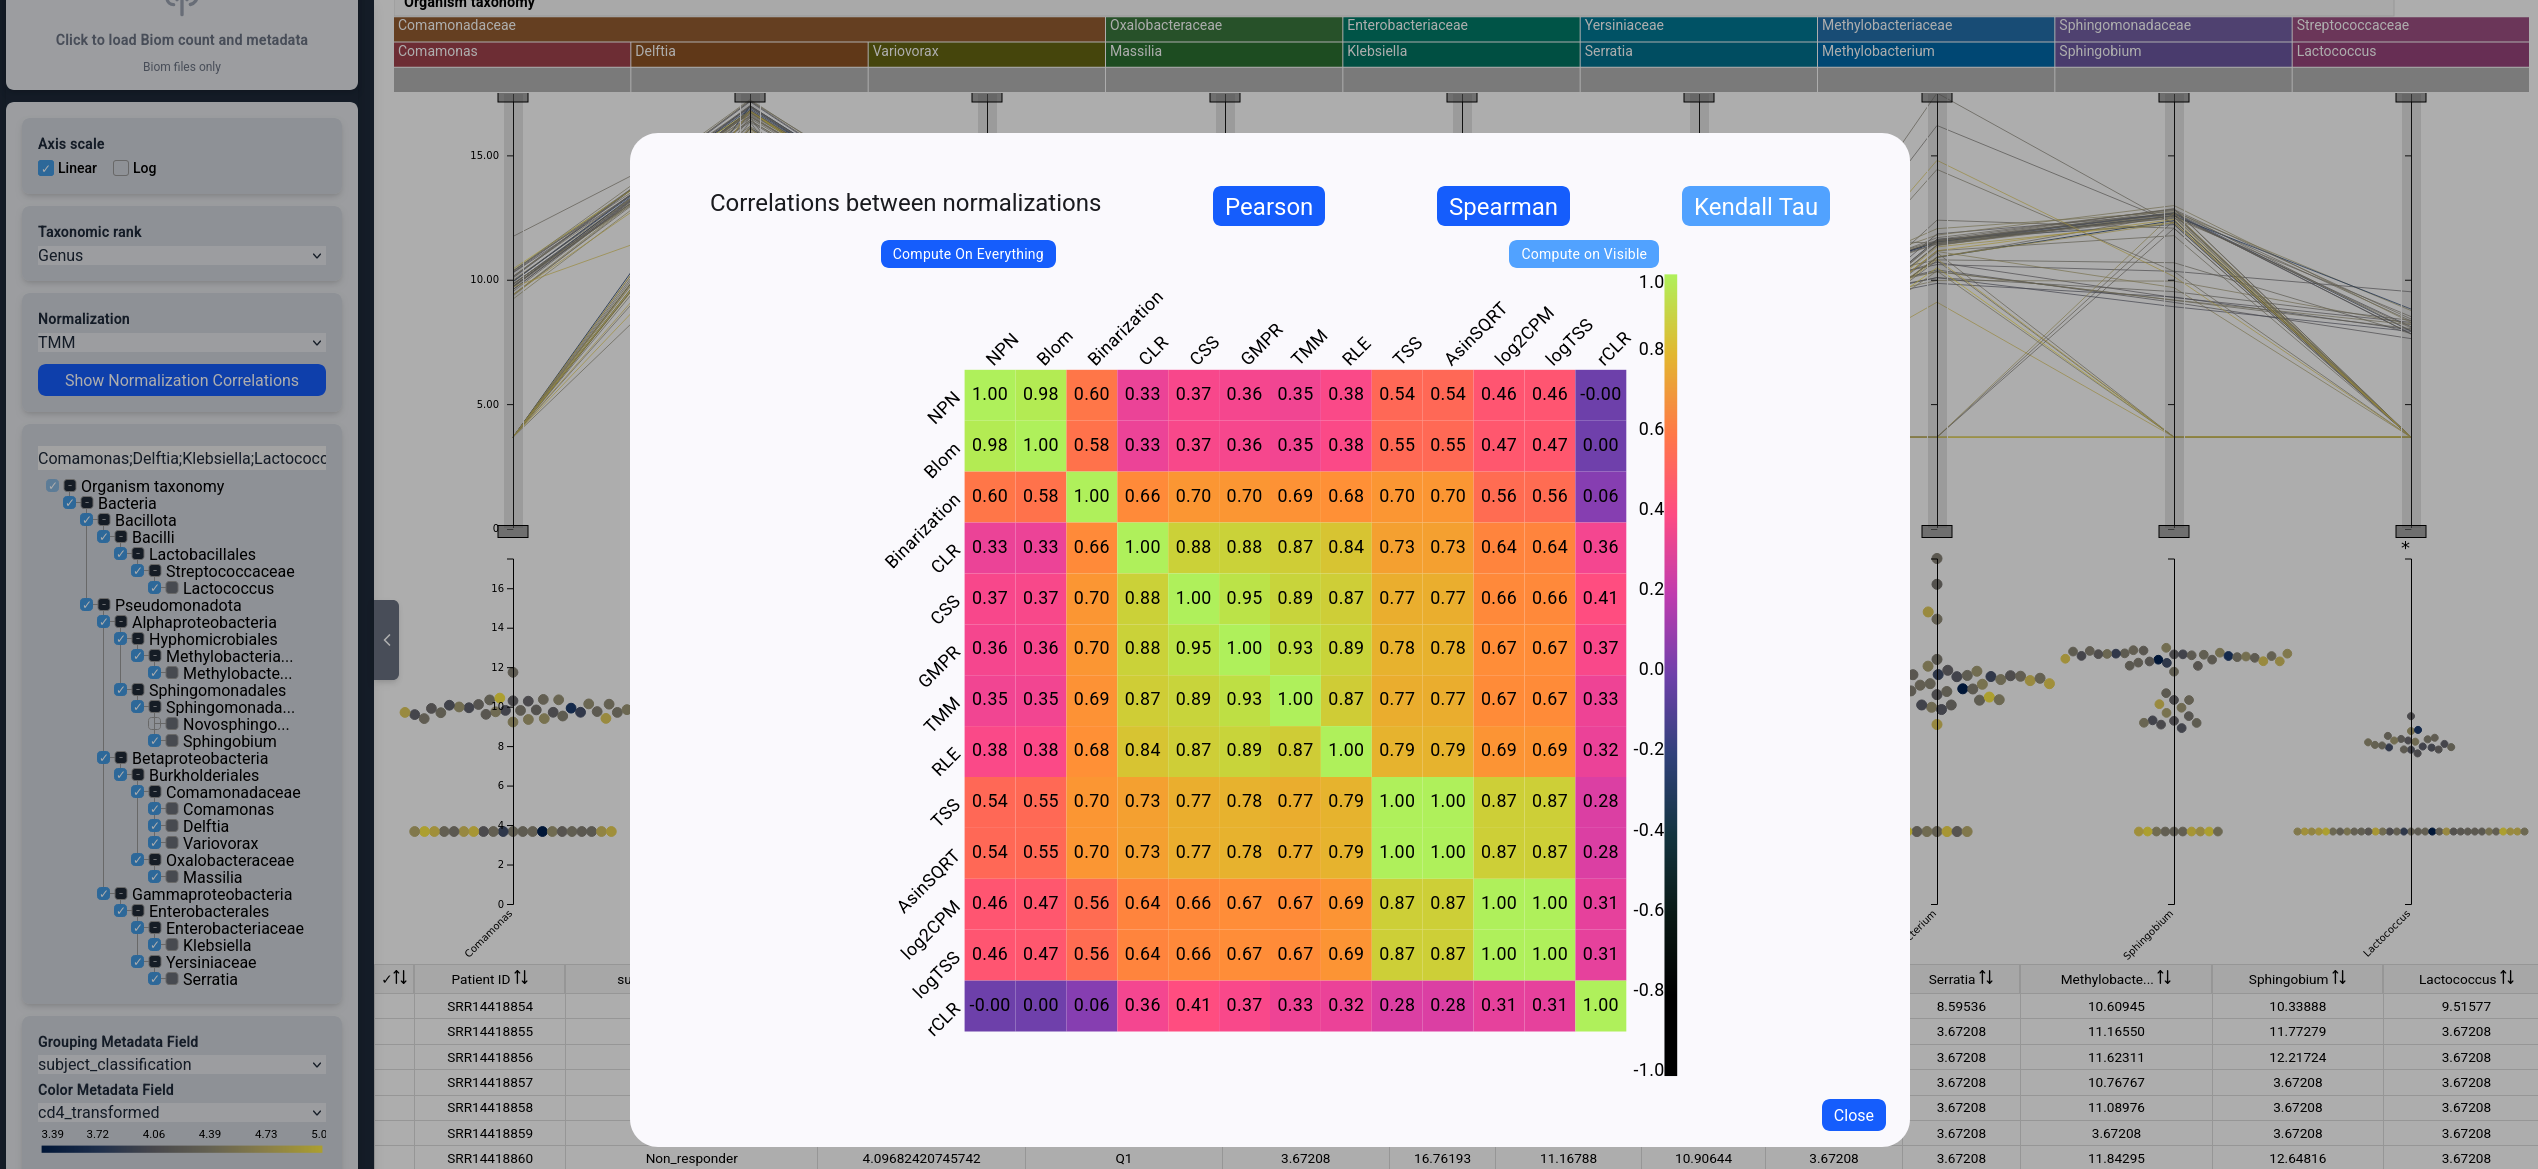
\includegraphics[width=\textwidth]{figures/v2/supp1.png}
    \caption{Comparison of normalization and transformation methods available in TaxaLoom for the Cleveland cohort, using the data presented in Figure~\ref{douek}. Pairwise correlations were computed between the vectorized abundance matrices obtained using each method. Similarity was evaluated using Kendall's tau correlation coefficient (shown), with Spearman's and Pearson's correlations also available through the interactive interface. Values closer to 1 indicate greater similarity between the abundance profiles obtained with the corresponding methods.}
    \label{supp:cor_heatmap}
\end{sidewaysfigure}



\subsection{Exploration of microbial profiles associated with immune response to cART}

The sample-level abundance profiles of the 9 selected genera in the Cleveland cohort in relation to immune response status and CD4 T-cell counts in Figure~\ref{douek}, using TMM normalization.


Figure~\ref{douek} 

\begin{figure}[htbp]
    \centering
    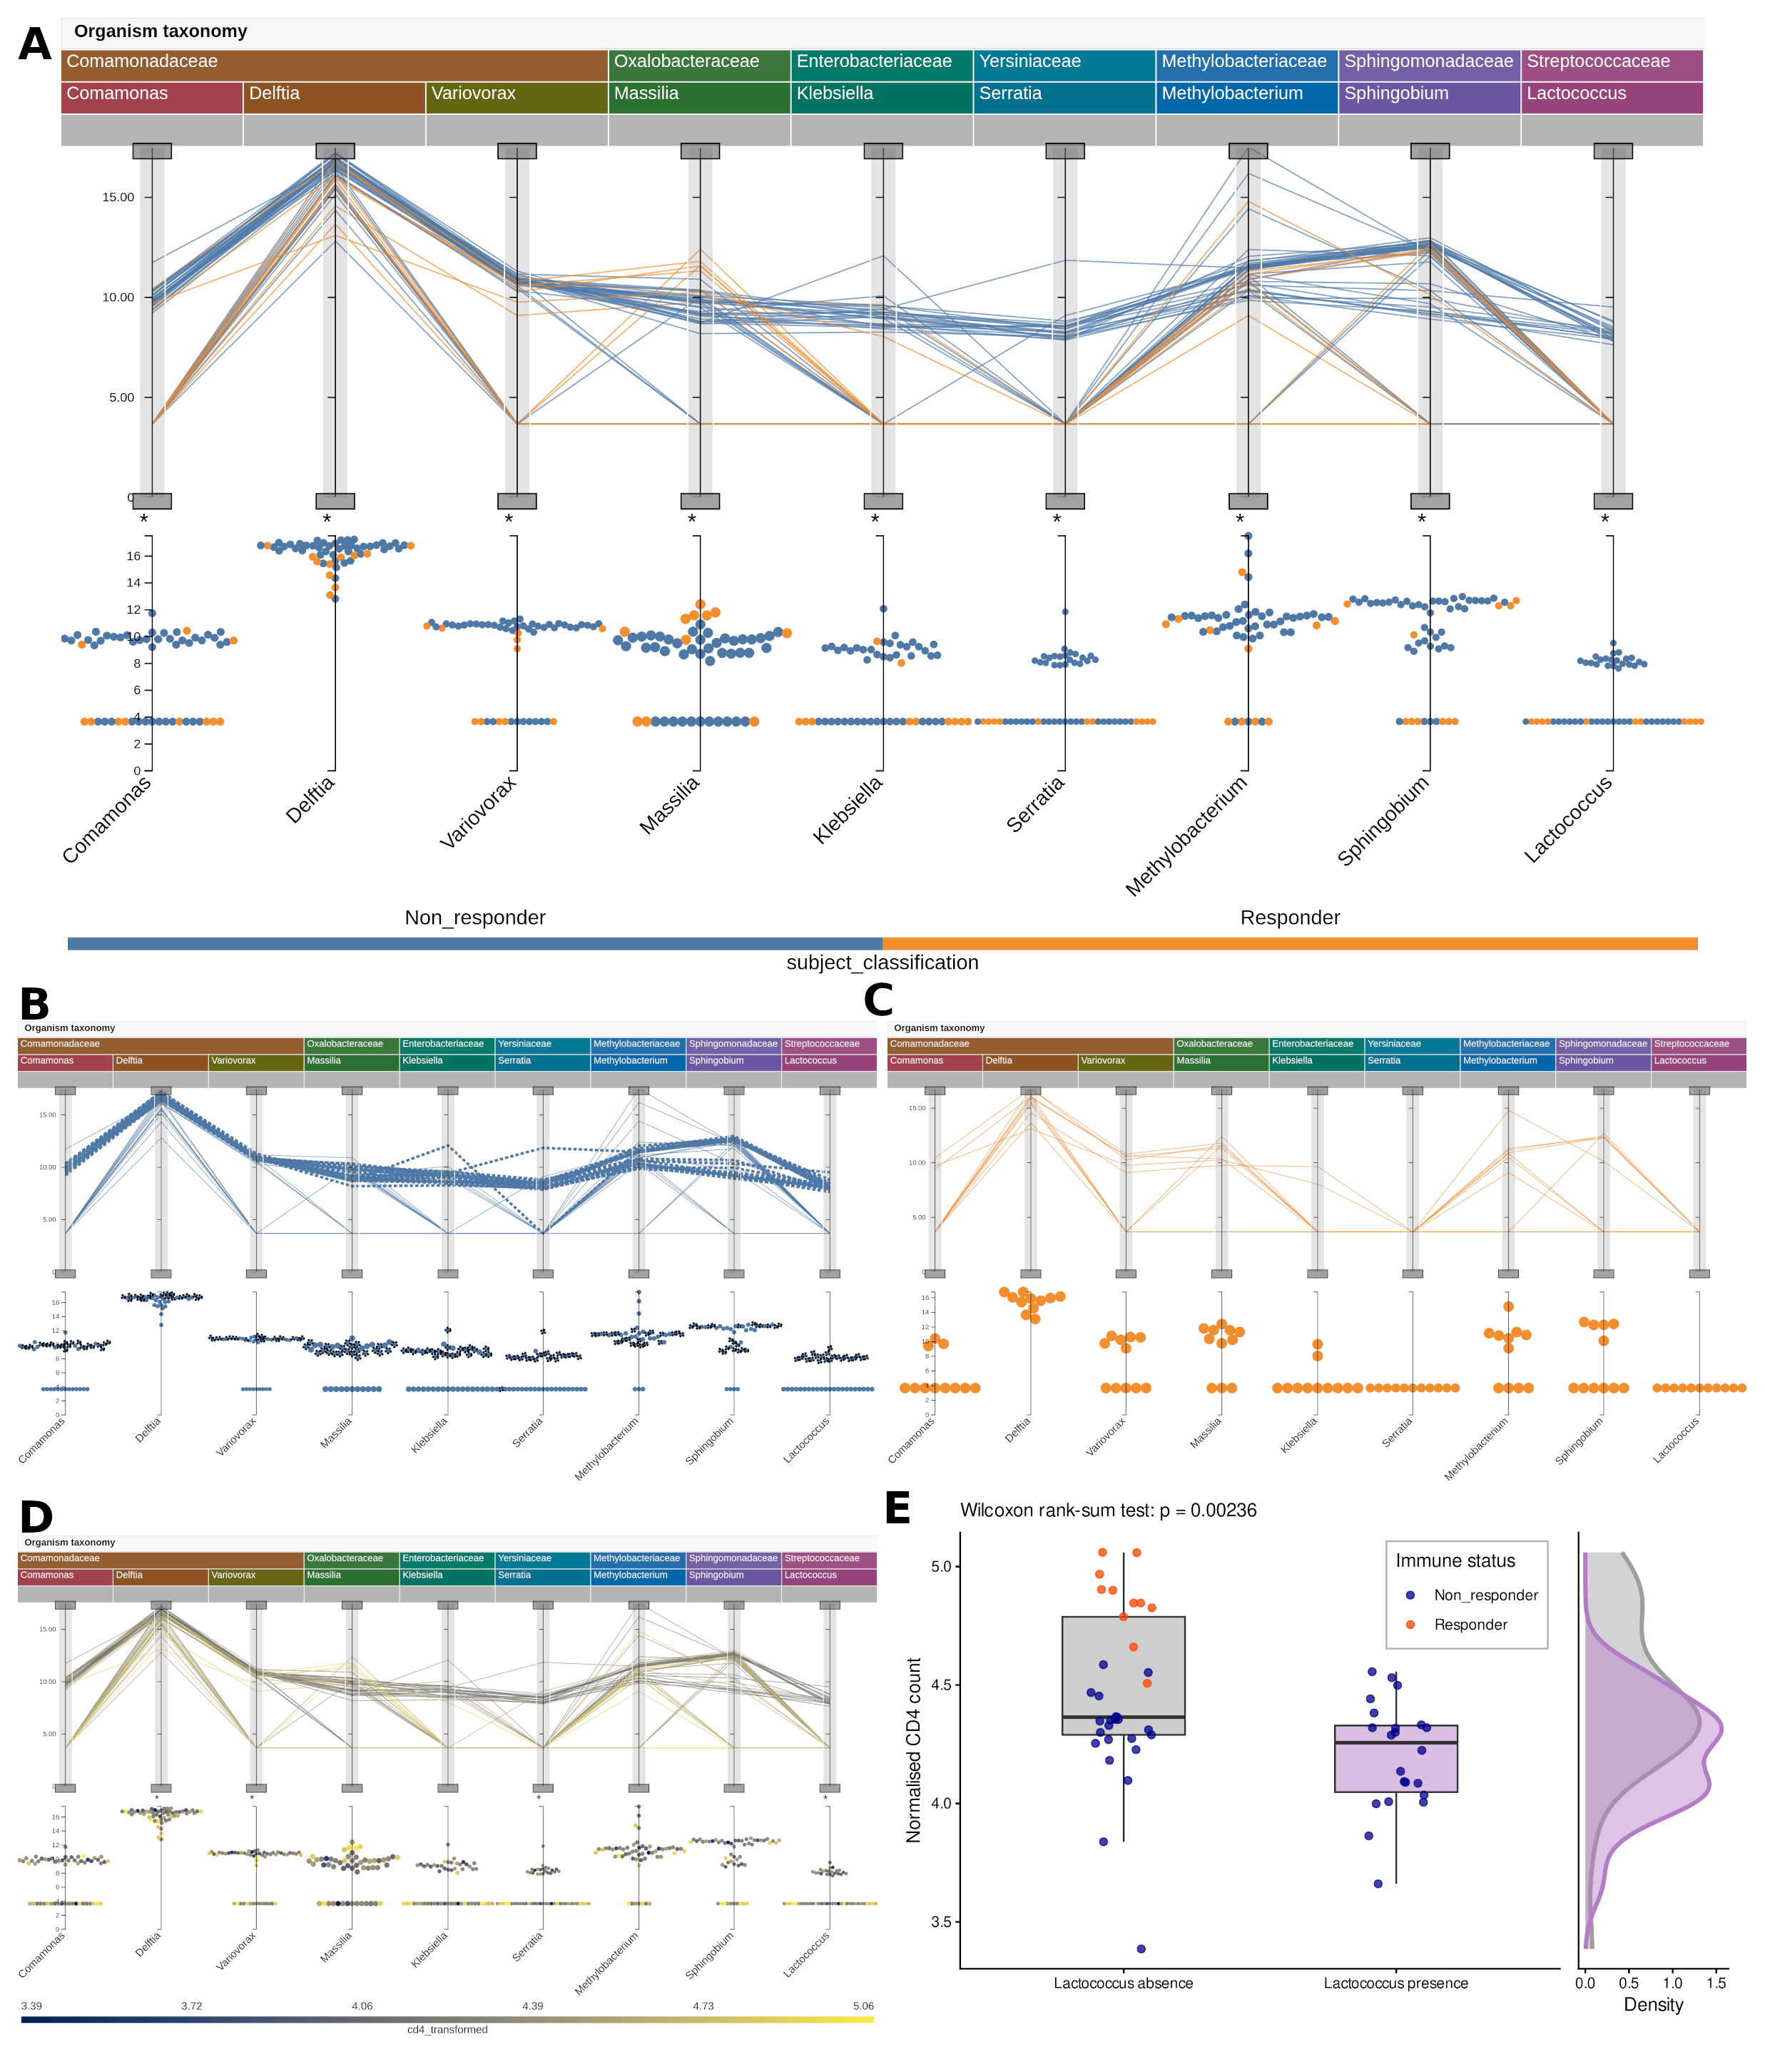
\includegraphics[width=\textwidth]{figures/v2/fig1.png}
    \caption{Exploration of microbial abundance profiles associated with immune response to cART in the Cleveland cohort. TaxaLoom visualization of 9 selected bacterial genera across 55 samples.
    (\textbf{A}) Samples coloured by immune response status (responders in orange, non-responders in blue).
    (\textbf{B}) Immune non-responders, with the 22 samples with non-zero \textit{Lactococcus} abundance highlighted by bold lines and circled swarm-plot points.
    (\textbf{C}) Immune responders.
    (\textbf{D}) Samples coloured by normalized CD4 T-cell counts.
    (\textbf{E}) Normalized CD4 T-cell counts according to \textit{Lactococcus} detection, with samples coloured by immune response status and density distributions shown on the right. Counts were lower in samples with non-zero \textit{Lactococcus} abundance (Wilcoxon rank-sum test, $W=540.5$, $p=0.00236$). Abundances were TMM-normalized in all panels.}
    \label{douek}
\end{figure}

Samples were initially coloured according to immune response status (Figure~\ref{douek}A). Separately examining immune non-responders (Figure~\ref{douek}B) and immune responders (Figure~\ref{douek}C) revealed substantial variability in abundance profiles within both groups. Among immune non-responders, interactive sample selection highlighted a subset of 22 samples with non-zero \textit{Lactococcus} abundance that shared similar abundance profiles across the displayed genera.

As immune response status is based on CD4 T-cell recovery, we further explored normalized CD4 T-cell counts as a quantitative variable (Figure~\ref{douek}D). The previously selected \textit{Lactococcus}-positive subset appeared to have lower CD4 T-cell counts. This visually identified pattern was subsequently evaluated statistically outside of TaxaLoom, showing significantly lower normalized CD4 T-cell counts in patients with non-zero \textit{Lactococcus} abundance compared with those in whom \textit{Lactococcus} was not detected (Wilcoxon rank-sum test, $W = 540.5$, $p = 0.002$; Figure~\ref{douek}E).

%This case study illustrates how interactive exploration can reveal heterogeneity within predefined clinical groups. In particular, the combination of categorical immune response status and quantitative CD4 T-cell measurements allowed us to identify a subset of patients with distinct microbial abundance profiles and explore their association with immune recovery. Although the observed association with \textit{Lactococcus} requires further validation, it demonstrates how sample-level visualization can guide the identification of patterns for subsequent statistical investigation.

This case study illustrates how interactive exploration can reveal heterogeneity within predefined clinical groups. In particular, the combination of categorical immune response status and quantitative CD4 T-cell measurements allowed us to identify a subset of patients with distinct microbial abundance profiles and explore their association with immune recovery. Although the observed association with \textit{Lactococcus} requires further validation, it demonstrates how sample-level visualization can guide the identification of patterns for subsequent statistical investigation. 

In the context of HIV infection, disruption of the gastrointestinal barrier can promote the translocation of microbial products and microorganisms into the systemic circulation, contributing to persistent immune activation and inflammation \citep{brenchley_microbial_2012,sandler_microbial_2012}. This mechanism is particularly relevant to the Cleveland cohort, where microbial signatures detected in blood were previously associated with systemic inflammation and CD4 T-cell recovery following combined antiretroviral therapy (cART) \citep{nganou-makamdop_translocated_2021}. The association observed here therefore raises the possibility that \textit{Lactococcus} detection may reflect a translocation-related process linked to poorer immune recovery, although the present data do not establish either the anatomical origin of these sequences or a causal relationship. The potential presence of translocated microbial signals in blood has also motivated probiotic interventions aimed at modulating the gut microbiota and reducing microbial translocation in individuals receiving cART \citep{dettorre_probiotics_2015}.


\subsubsection{Identification of sequencing-associated microbial patterns in TCGA}

Using TaxaLoom, we explored TCGA microbial profiles together with technical metadata to investigate sample-level abundance patterns associated with sequencing centre and read length (Figure~\ref{fig:contamination}). To obtain this figure, we further show in Figure~\ref{fig:explo_conta} how we successively selected taxa, started from the phylum down to genus and species, where interesting patterns could be easily identified. 

We started this exploration with enteric bacteria from the order \textit{Enterobacterales}, shown in Figure~\ref{fig:explo_conta}A, as these taxa represented plausible candidates for contamination-related signals. This allowed us to identify \textit{Escherichia coli} and \textit{Escherichia albertii}, together with \textit{Klebsiella pneumoniae} and \textit{Salmonella enterica}, as exhibiting marked differences in abundance according to sequencing centre.


\begin{figure}[!h]
    \centering
    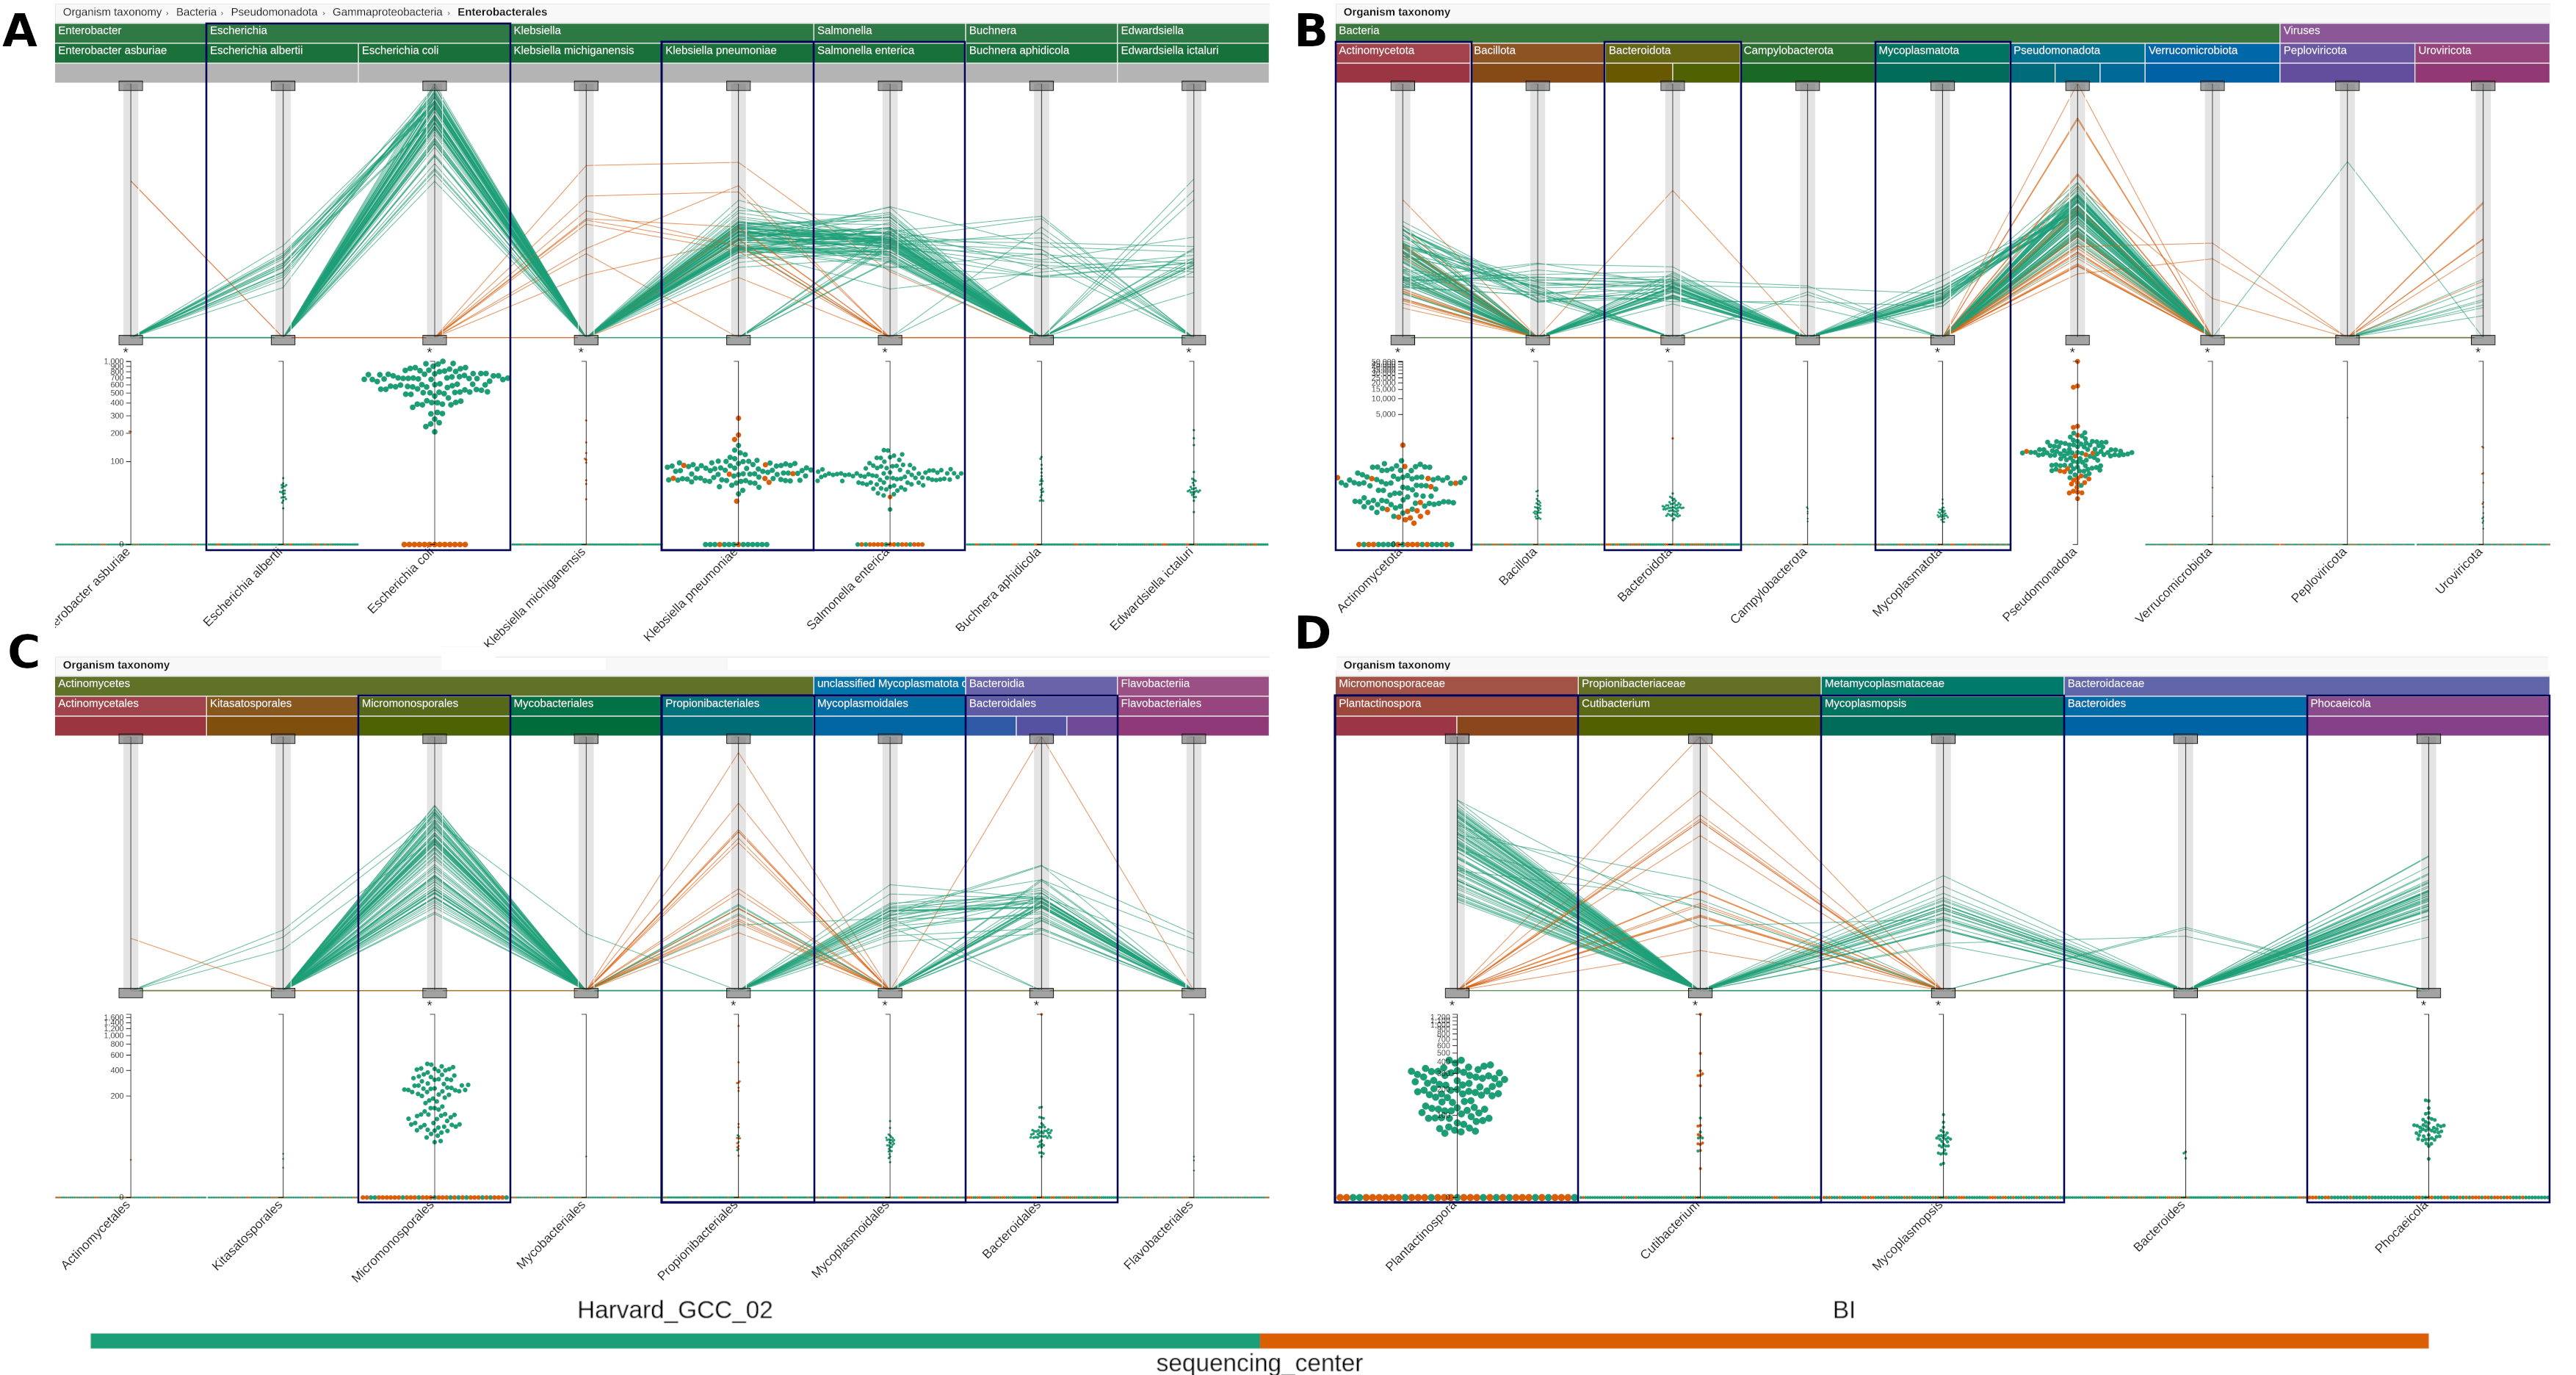
\includegraphics[width=\textwidth]{figures/v2/fig3.png}
    \caption{Progressive taxonomic filtering of TCGA-THCA microbial profiles using TaxaLoom. Taxonomic branches were successively filtered to focus on taxa exhibiting sequencing-associated abundance patterns. The selected taxa for Figure~\ref{fig:contamination} are highlighted with a dark blue rectangle.
    (\textbf{A}) Separate exploration of genera belonging to the order \textit{Enterobacterales}, with selected taxa retained for Figure~\ref{fig:contamination}.
    (\textbf{B}) Filtering starting at the phylum level, where \textit{Actinomycetota}, \textit{Bacteroidota}, and \textit{Mycoplasmatota} were retained for further exploration at the order level.
    (\textbf{C}) Order-level visualization, from which \textit{Micromonosporales}, \textit{Propionibacteriales}, \textit{Mycoplasmoidales}, and \textit{Bacteroidales} were retained.
    (\textbf{D}) Genus-level visualization, with \textit{Mycoplasmopsis}, \textit{Plantactinospora}, \textit{Cutibacterium}, and \textit{Phocaeicola} retained for Figure~\ref{fig:contamination}. Abundances were normalized using GMPR and displayed on a logarithmic scale.}
\label{fig:explo_conta}
\end{figure}


To identify similar patterns elsewhere in the taxonomy, we progressively filtered the taxonomic tree using TaxaLoom starting from the phylum level (Figure~\ref{fig:explo_conta}B). Branches were successively removed to focus on \textit{Actinomycetota}, \textit{Bacteroidota}, and \textit{Mycoplasmatota}. We chose not to keep \textit{Pseudomonadota} for further exploration, as a lower taxonomic group, the \textit{Enterobacterales} family was already shown in Figure Figure~\ref{fig:explo_conta}A. Therefore, the retained branches were explored at increasingly specific taxonomic levels, from orders (Figure~\ref{fig:explo_conta}C) to genera (Figure~\ref{fig:explo_conta}D), where the visualization was further restricted to \textit{Plantactinospora}, \textit{Cutibacterium}, \textit{Mycoplasmopsis},  and \textit{Phocaeicola}. This progressive filtering ultimately reduced the visualization to species belonging to these mentioned genera in Figure~\ref{fig:contamination}.

The final visualization contained nine species: \textit{Salmonella enterica}, \textit{Klebsiella pneumoniae}, \textit{Escherichia coli}, \textit{Escherichia albertii}, two \textit{Plantactinospora} species, \textit{Cutibacterium acnes}, \textit{Phocaeicola dorei}, and \textit{Mycoplasmopsis bovis}. Their abundance profiles were compared to detect eventual association with sequencing centre or read length as analysed in Figure~\ref{fig:contamination}A-B.

Marked sample-specific patterns were observed across the nine selected species (Figure~\ref{fig:contamination}). The clearest pattern was observed for \textit{Escherichia coli}: all samples from \texttt{Harvard\_GCC\_02} had non-zero \textit{E. coli} abundance, whereas \textit{E. coli} was not detected in any sample sequenced at \texttt{BI} (Figure~\ref{fig:contamination}A). Sequencing centre was completely associated with read length, with all \texttt{Harvard\_GCC\_02} samples having 51-bp reads and \texttt{BI} samples having 101 or 151-bp reads shown in blue and yellow in Figure~\ref{fig:contamination}B.

The concordance between microbial abundance profiles and these technical variables indicates that technical effects may contribute to the observed patterns. For \texttt{Harvard\_GCC\_02}, the high abundance of \textit{E. coli} and related \textit{Enterobacterales} could reflect contamination introduced during sample processing. However, the complete association between sequencing centre and read length prevents these effects from being disentangled. The shorter 51-bp reads may also provide lower taxonomic resolution, potentially contributing to classifications among closely related Enterobacterales such as \textit{K. pneumoniae}, \textit{S. enterica}, and \textit{E. albertii}. Conversely, \texttt{BI} samples showed higher abundance of \textit{C. acnes}, a common skin-associated contaminant also identified as a potential contaminant in TCGA data by \citet{ge_comprehensive_2025}. No clear explanation was identified for the sequencing-associated patterns observed for \textit{M. bovis}, \textit{P. dorei}, and \textit{Plantactinospora} spp.


\begin{figure}[!h]
    \centering
    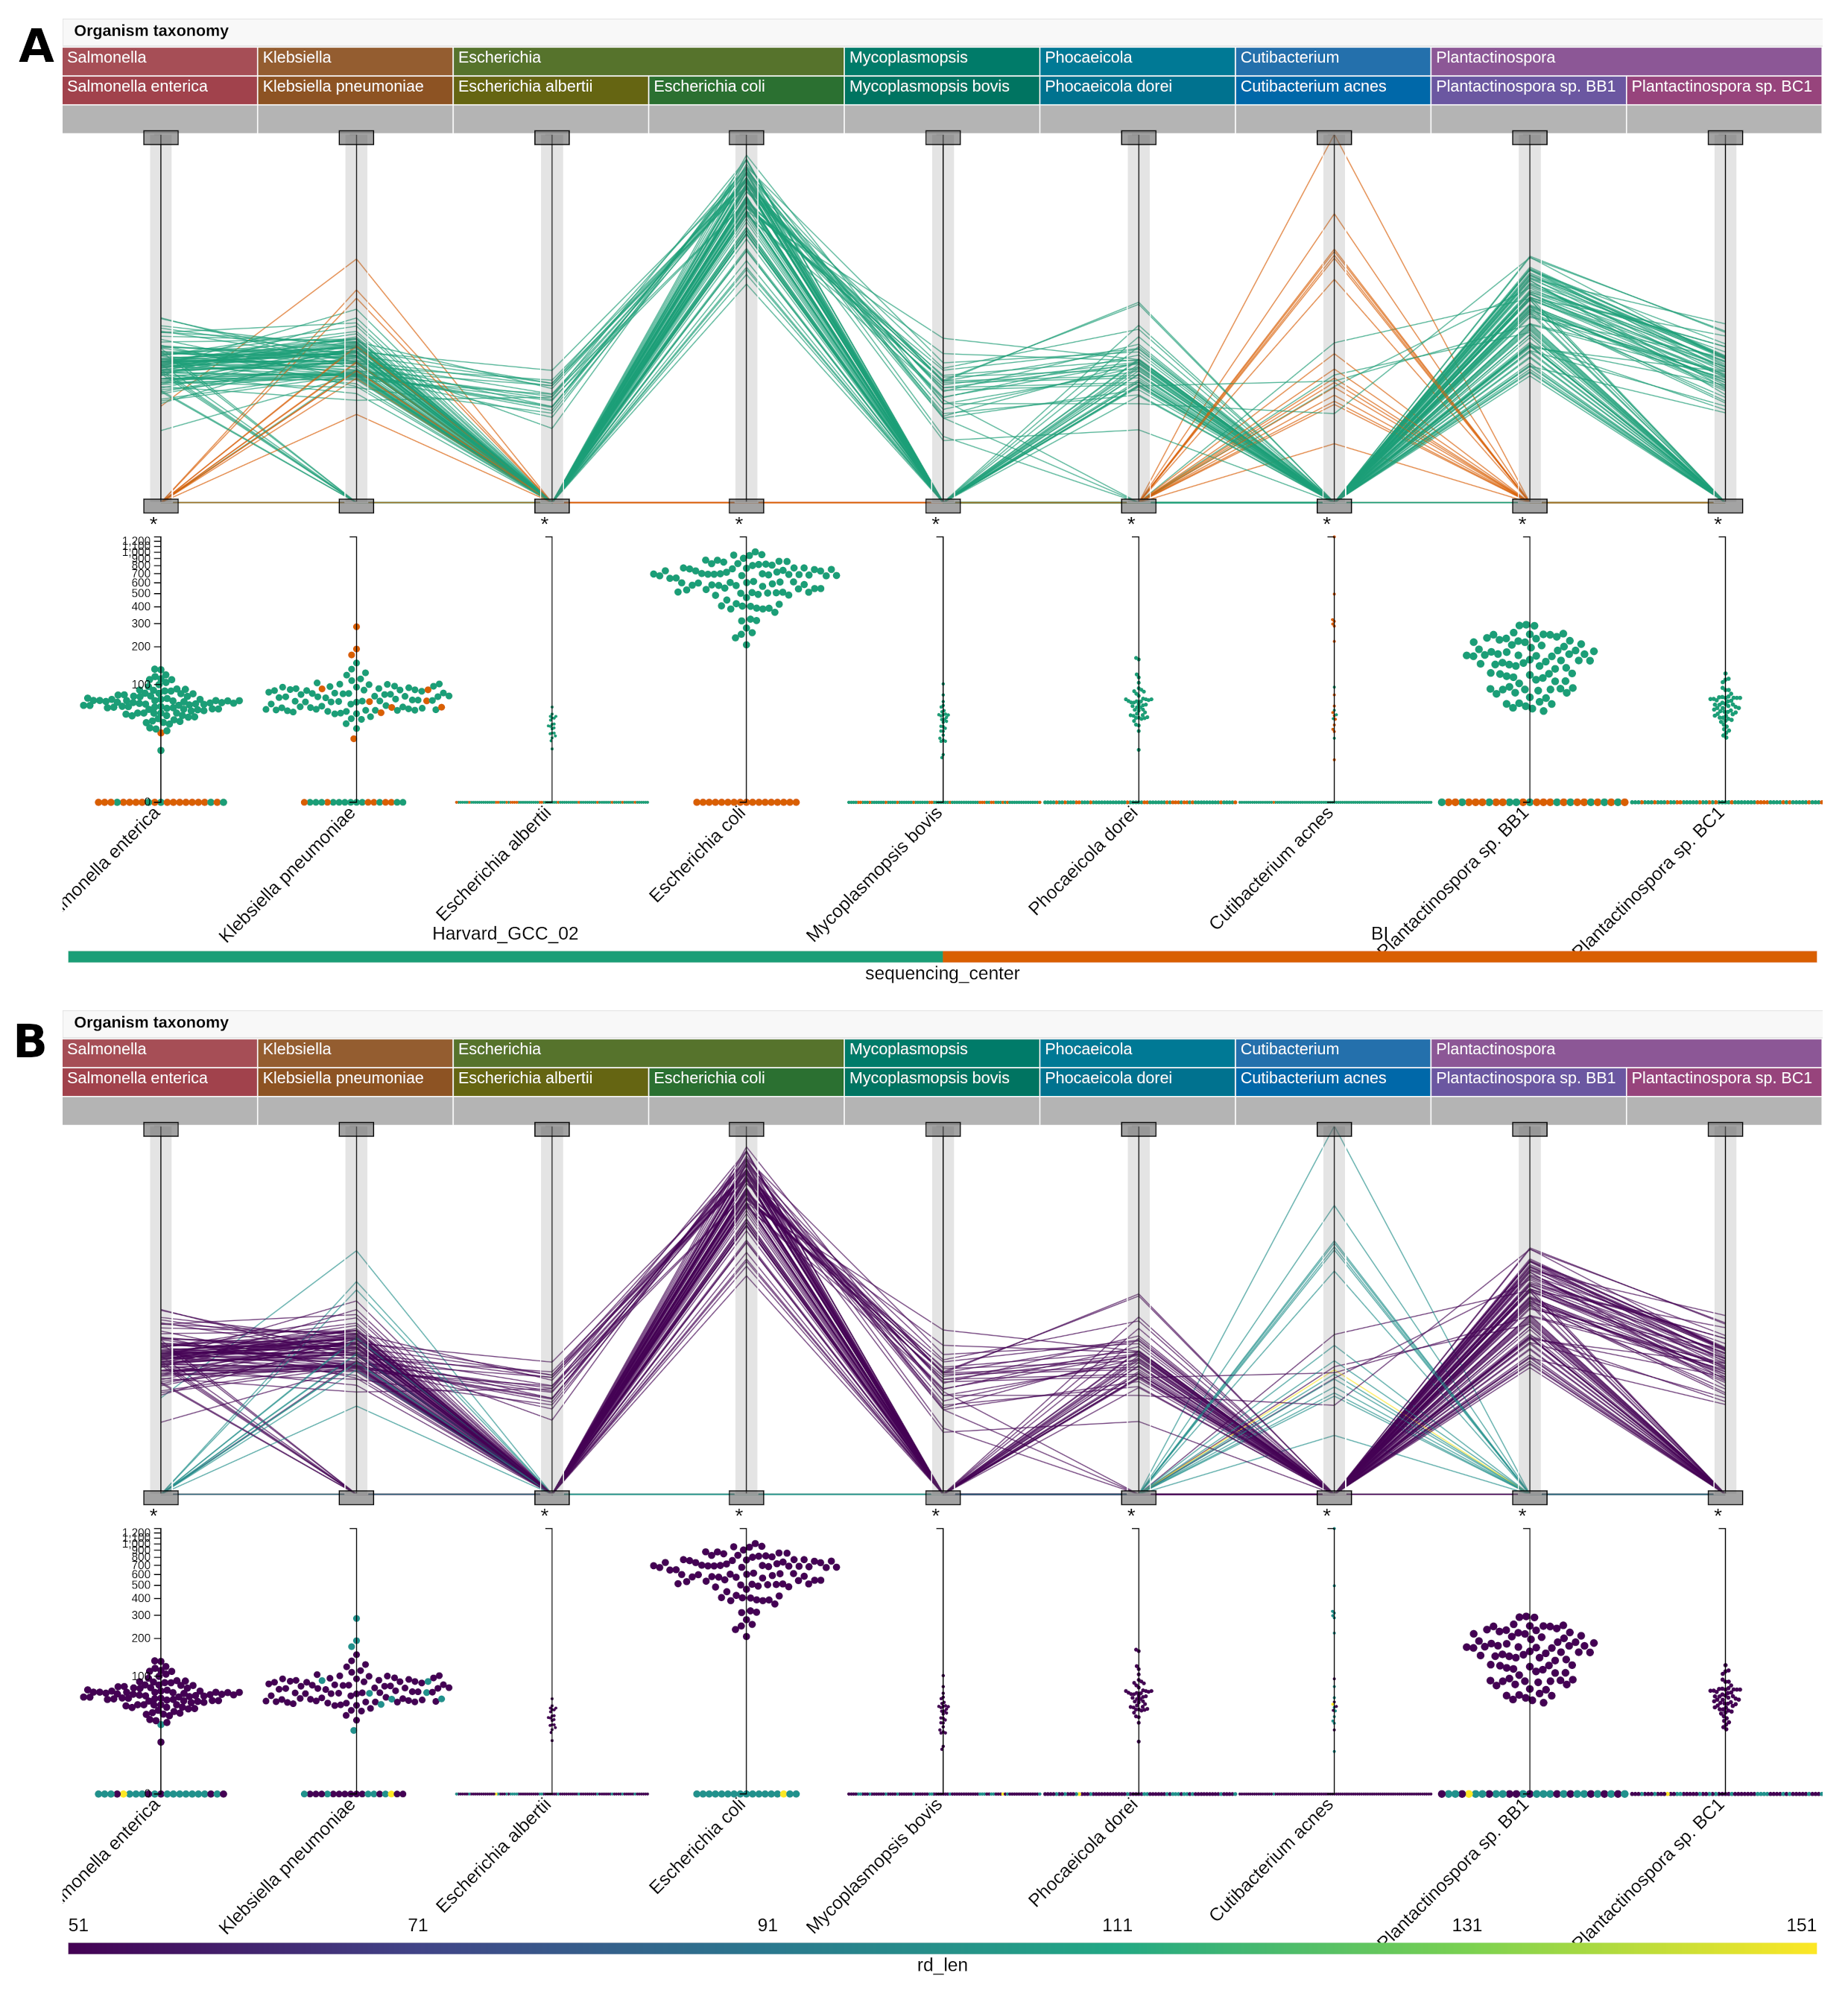
\includegraphics[width=\textwidth]{figures/v2/fig2.png}
      \caption{Sample-level microbial abundance patterns associated with technical variables in TCGA-THCA. TaxaLoom visualization of nine selected microbial species across 122 TCGA-THCA \texttt{Primary Tumor} samples. Samples are coloured according to (\textbf{A}) sequencing centre, with \texttt{Harvard\_GCC\_02} shown in green and \texttt{BI} in orange, and (\textbf{B}) read length (51, 101, or 151 bp). Abundances were normalized using GMPR and displayed on a logarithmic scale.}

    \label{fig:contamination}
\end{figure}



\section{Conclusion}\label{sec4}

The exploration of microbial taxonomic abundance profiles requires considering the hierarchical structure of microbial taxonomy, the characteristics of abundance distributions, and the integration of sample metadata. As the number of taxa and samples increases, examining these different aspect simultaneously becomes increasingly challenging. To address these challenges, we developed TaxaLoom, an interactive web-based application combining taxonomic navigation, sample-level visualization, metadata integration, and the comparison of normalization and transformation methods. The two case studies illustrate how TaxaLoom can support the exploration of biological patterns and the identification of potential sequencing-related artefacts. By providing complementary visual representations of microbial abundance data within a common interface, TaxaLoom facilitates exploratory analysis and the identification of patterns that may warrant further investigation.


\section*{Availability and requirements}\label{sec6}

TaxaLoom is an open-source, platform-independent web application developed using Angular and TypeScript. It can be accessed through modern desktop web browsers, including Firefox, Chromium, Google Chrome, Microsoft Edge, and GNOME Web. The source code is available at \url{INSERT_GITHUB_URL} under the MIT license, with no restrictions on non-academic use. Local installation and development require npm and Angular CLI, tested with versions 11.19.0 and 21, respectively. Compatibility with mobile browsers has not been evaluated.


\section*{Abbreviations}

ALR: Additive log-ratio; AsinSQRT: Arcsine square-root transformation; BIOM: Biological Observation Matrix; cART: Combination antiretroviral therapy; CD4: Cluster of differentiation 4; CLR: Centered log-ratio; CSS: Cumulative-sum scaling; DNA: Deoxyribonucleic acid; GMPR: Geometric mean of pairwise ratios; HIV: Human immunodeficiency virus; HMP: Human Microbiome Project; NPN: Non-paranormal transformation; OTU: Operational taxonomic unit; PCoA: Principal coordinates analysis; rCLR: Robust centered log-ratio; RLE: Relative log expression; RNA: Ribonucleic acid; rRNA: Ribosomal RNA; TCGA: The Cancer Genome Atlas; TCGA-THCA: The Cancer Genome Atlas Thyroid Carcinoma; TMM: Trimmed mean of M-values; TSS: Total-sum scaling.


\section*{Authors' contributions}

AC curated the data and conceived the case studies. AC and PT wrote the manuscript. RB conceived and designed the software architecture. JC and SDB implemented the initial prototype of TaxaLoom under the supervision of AC, PT, and RB, and FL continued its development and implemented the version presented in this work. AC, PT, RB, FL, and RT contributed to discussions that shaped the conceptual development and direction of TaxaLoom.


\backmatter

%\section*{Abbreviations}

%\begin{description}
%  \item[mRNA:] Messenger ribonucleic acid
%  \item[RNA:] Ribonucleic acid
%\end{description}


\bibliography{sn-bibliography}



%\bmhead{Acknowledgements}

%\section*{Declarations}

%\begin{itemize}
%\item Funding
%\item Conflict of interest/Competing interests (check journal-specific guidelines for which heading to use)
%\item Ethics approval and consent to participate
%\item Consent for publication
%\item Data availability 
%\item Materials availability
%\item Code availability 
%\item Author contribution
%\end{itemize}


\clearpage


\begin{bibunit}[apalike]

\setcounter{page}{1}


\begin{appendices}


%\section{Supplementary Figures}\label{secA}
\setcounter{figure}{0}
\renewcommand{\thefigure}{S\arabic{figure}}



%\begin{figure}[hbtp]
%    \centering
%    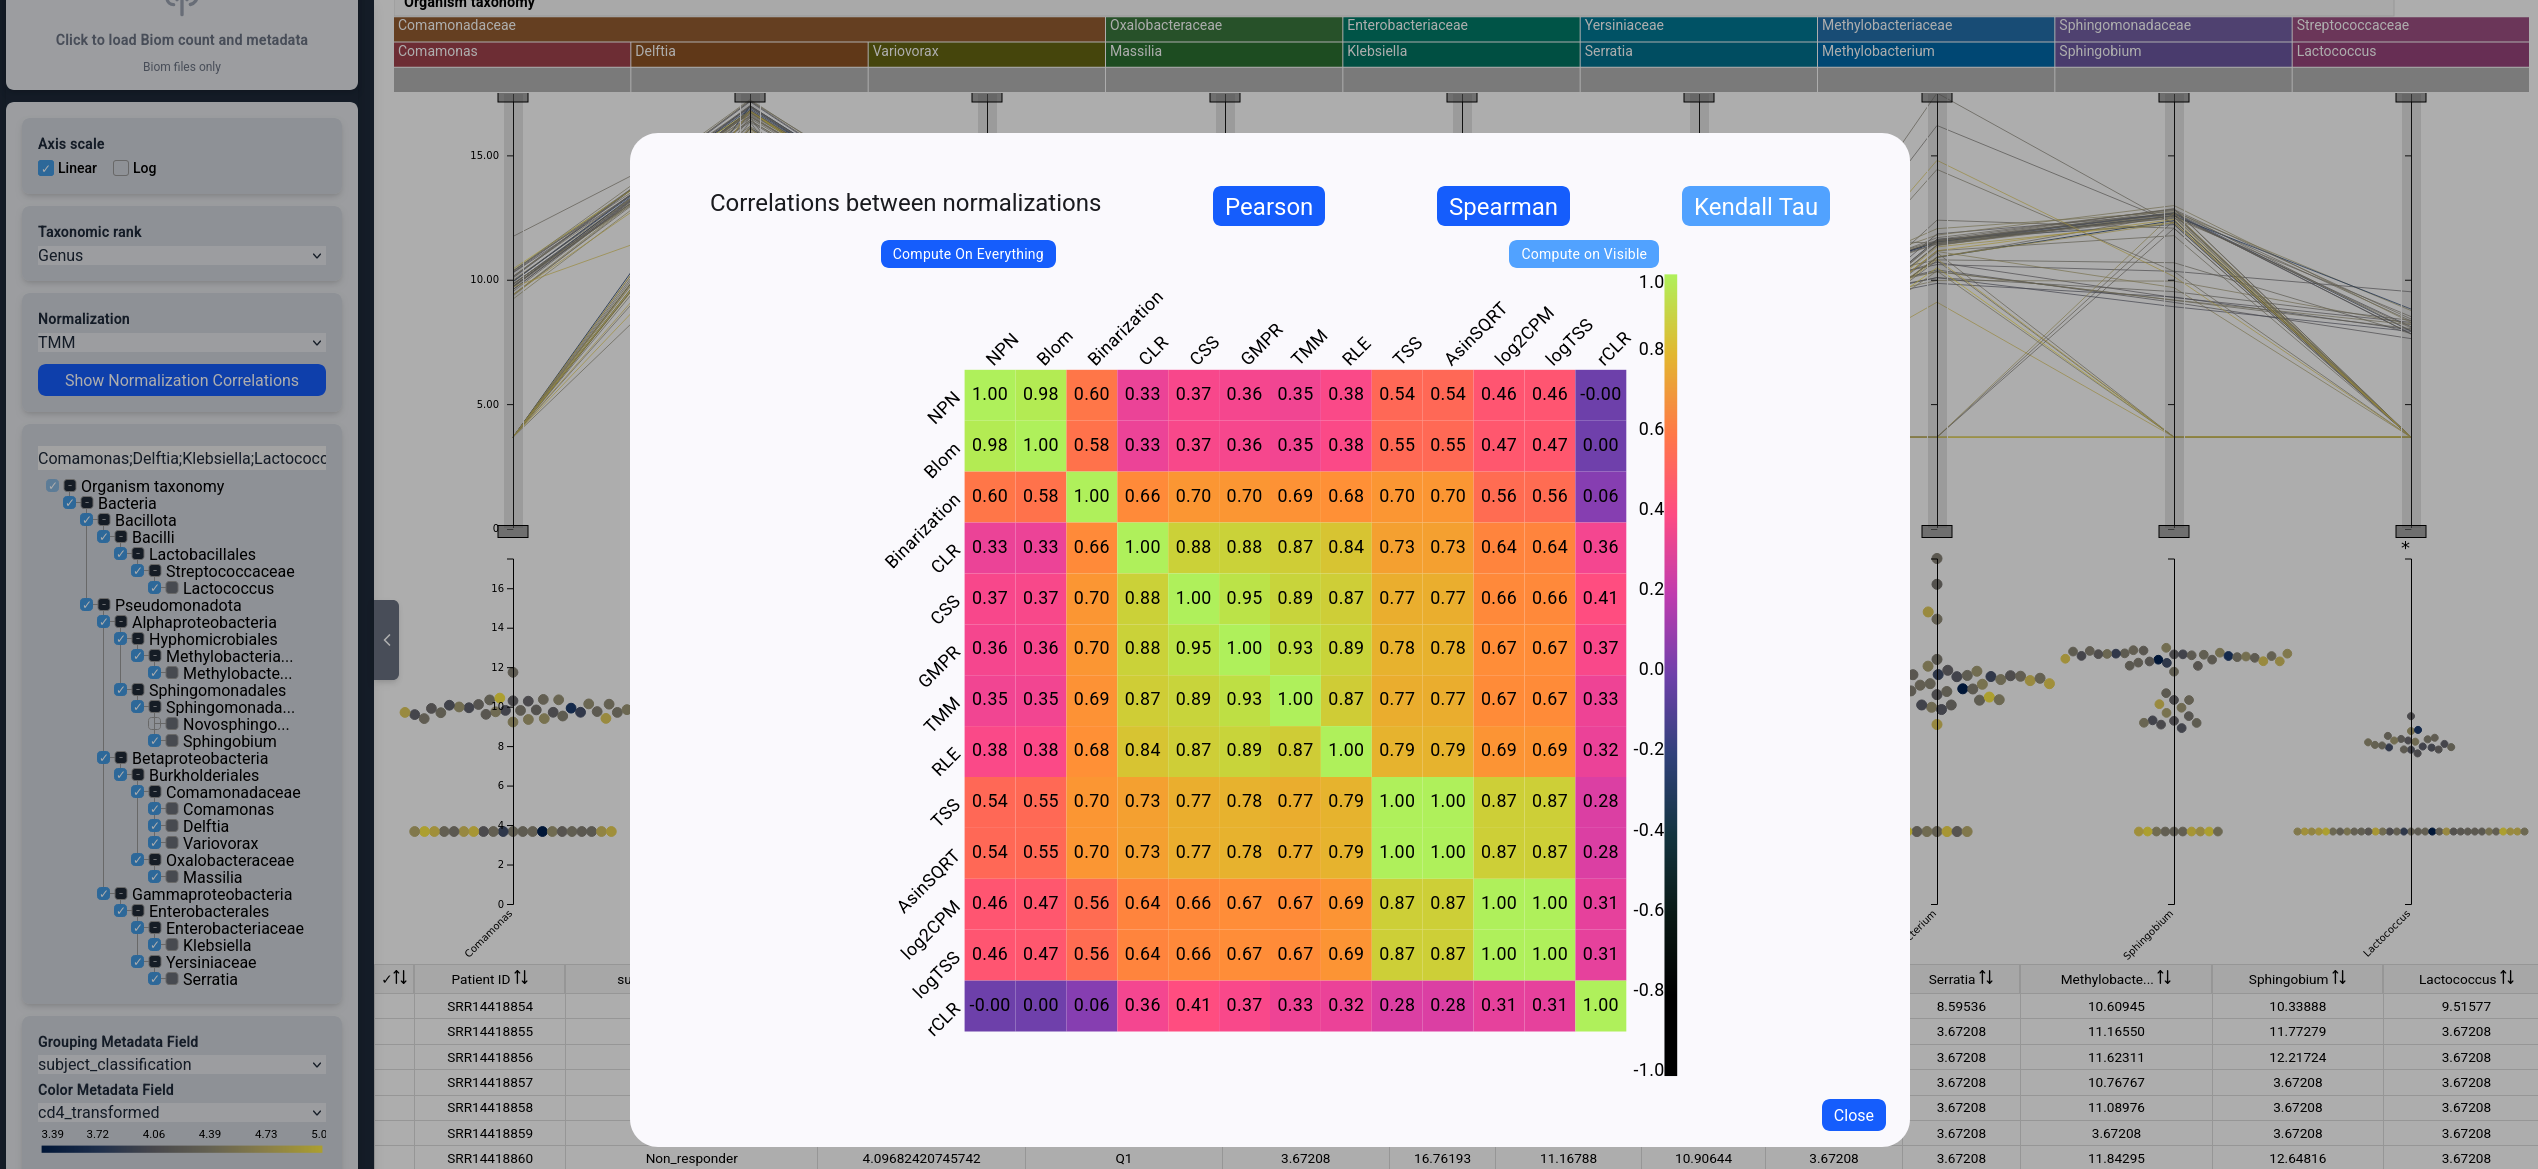
\includegraphics[width=\textwidth]{figures/v2/supp1.png}
%\caption{Comparison of normalization and transformation methods available in TaxaLoom for the Cleveland cohort, using the data presented in Figure~\ref{douek}. Pairwise correlations were computed between the vectorized abundance matrices obtained using each method. Similarity was evaluated using Kendall's correlation coefficient (shown), with Spearman's and Pearson's correlations also available through the interactive interface. Values closer to 1 indicate greater similarity between the abundance profiles obtained with the corresponding methods.}
%    \label{supp:cor_heatmap}
%\end{figure}


%\begin{figure}[htbp]
%    \centering
%    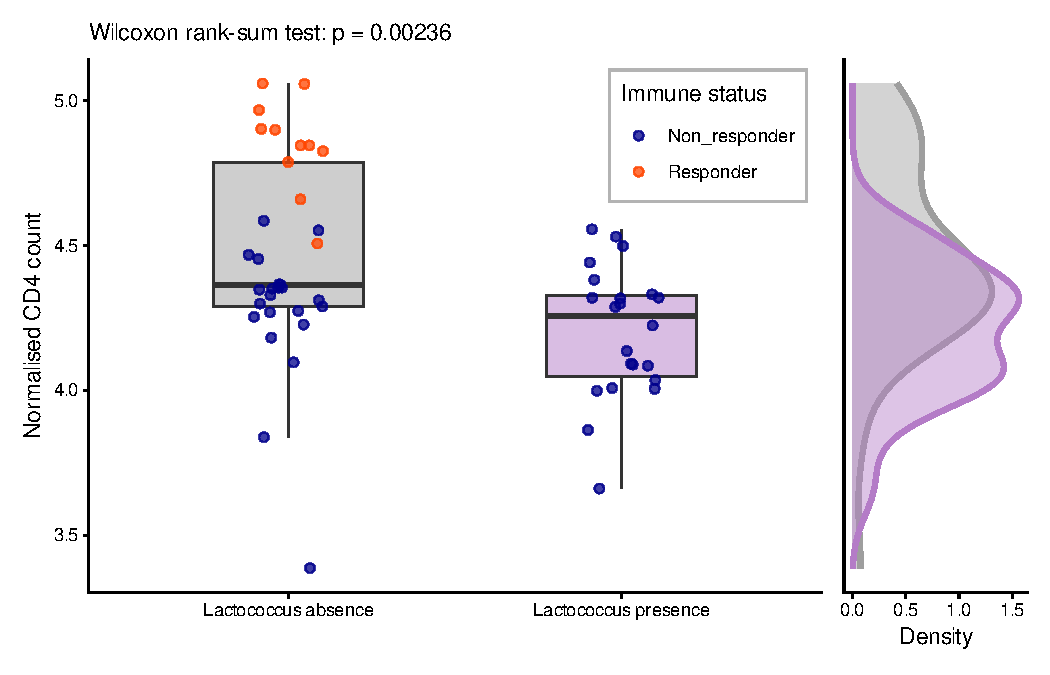
\includegraphics[width=\textwidth]{figures/supp1.pdf}
%    \caption{Boxplots of normalized CD4 T-cell counts according to \textit{Lactococcus} detection in the Cleveland cohort. Distribution of normalized CD4 T-cell counts in samples with and without detected \textit{Lactococcus}. Individual samples are coloured according to immune response status. Boxplots summarize the distribution within each group, with corresponding density distributions shown on the right. Normalized CD4 T-cell counts were significantly lower in samples with non-zero \textit{Lactococcus} abundance (Wilcoxon rank-sum test, $W=540.5$, $p=0.00236$).}    
%\label{figsupp:boxplots}
%\end{figure}



%\begin{figure}[htbp]
%    \centering
%    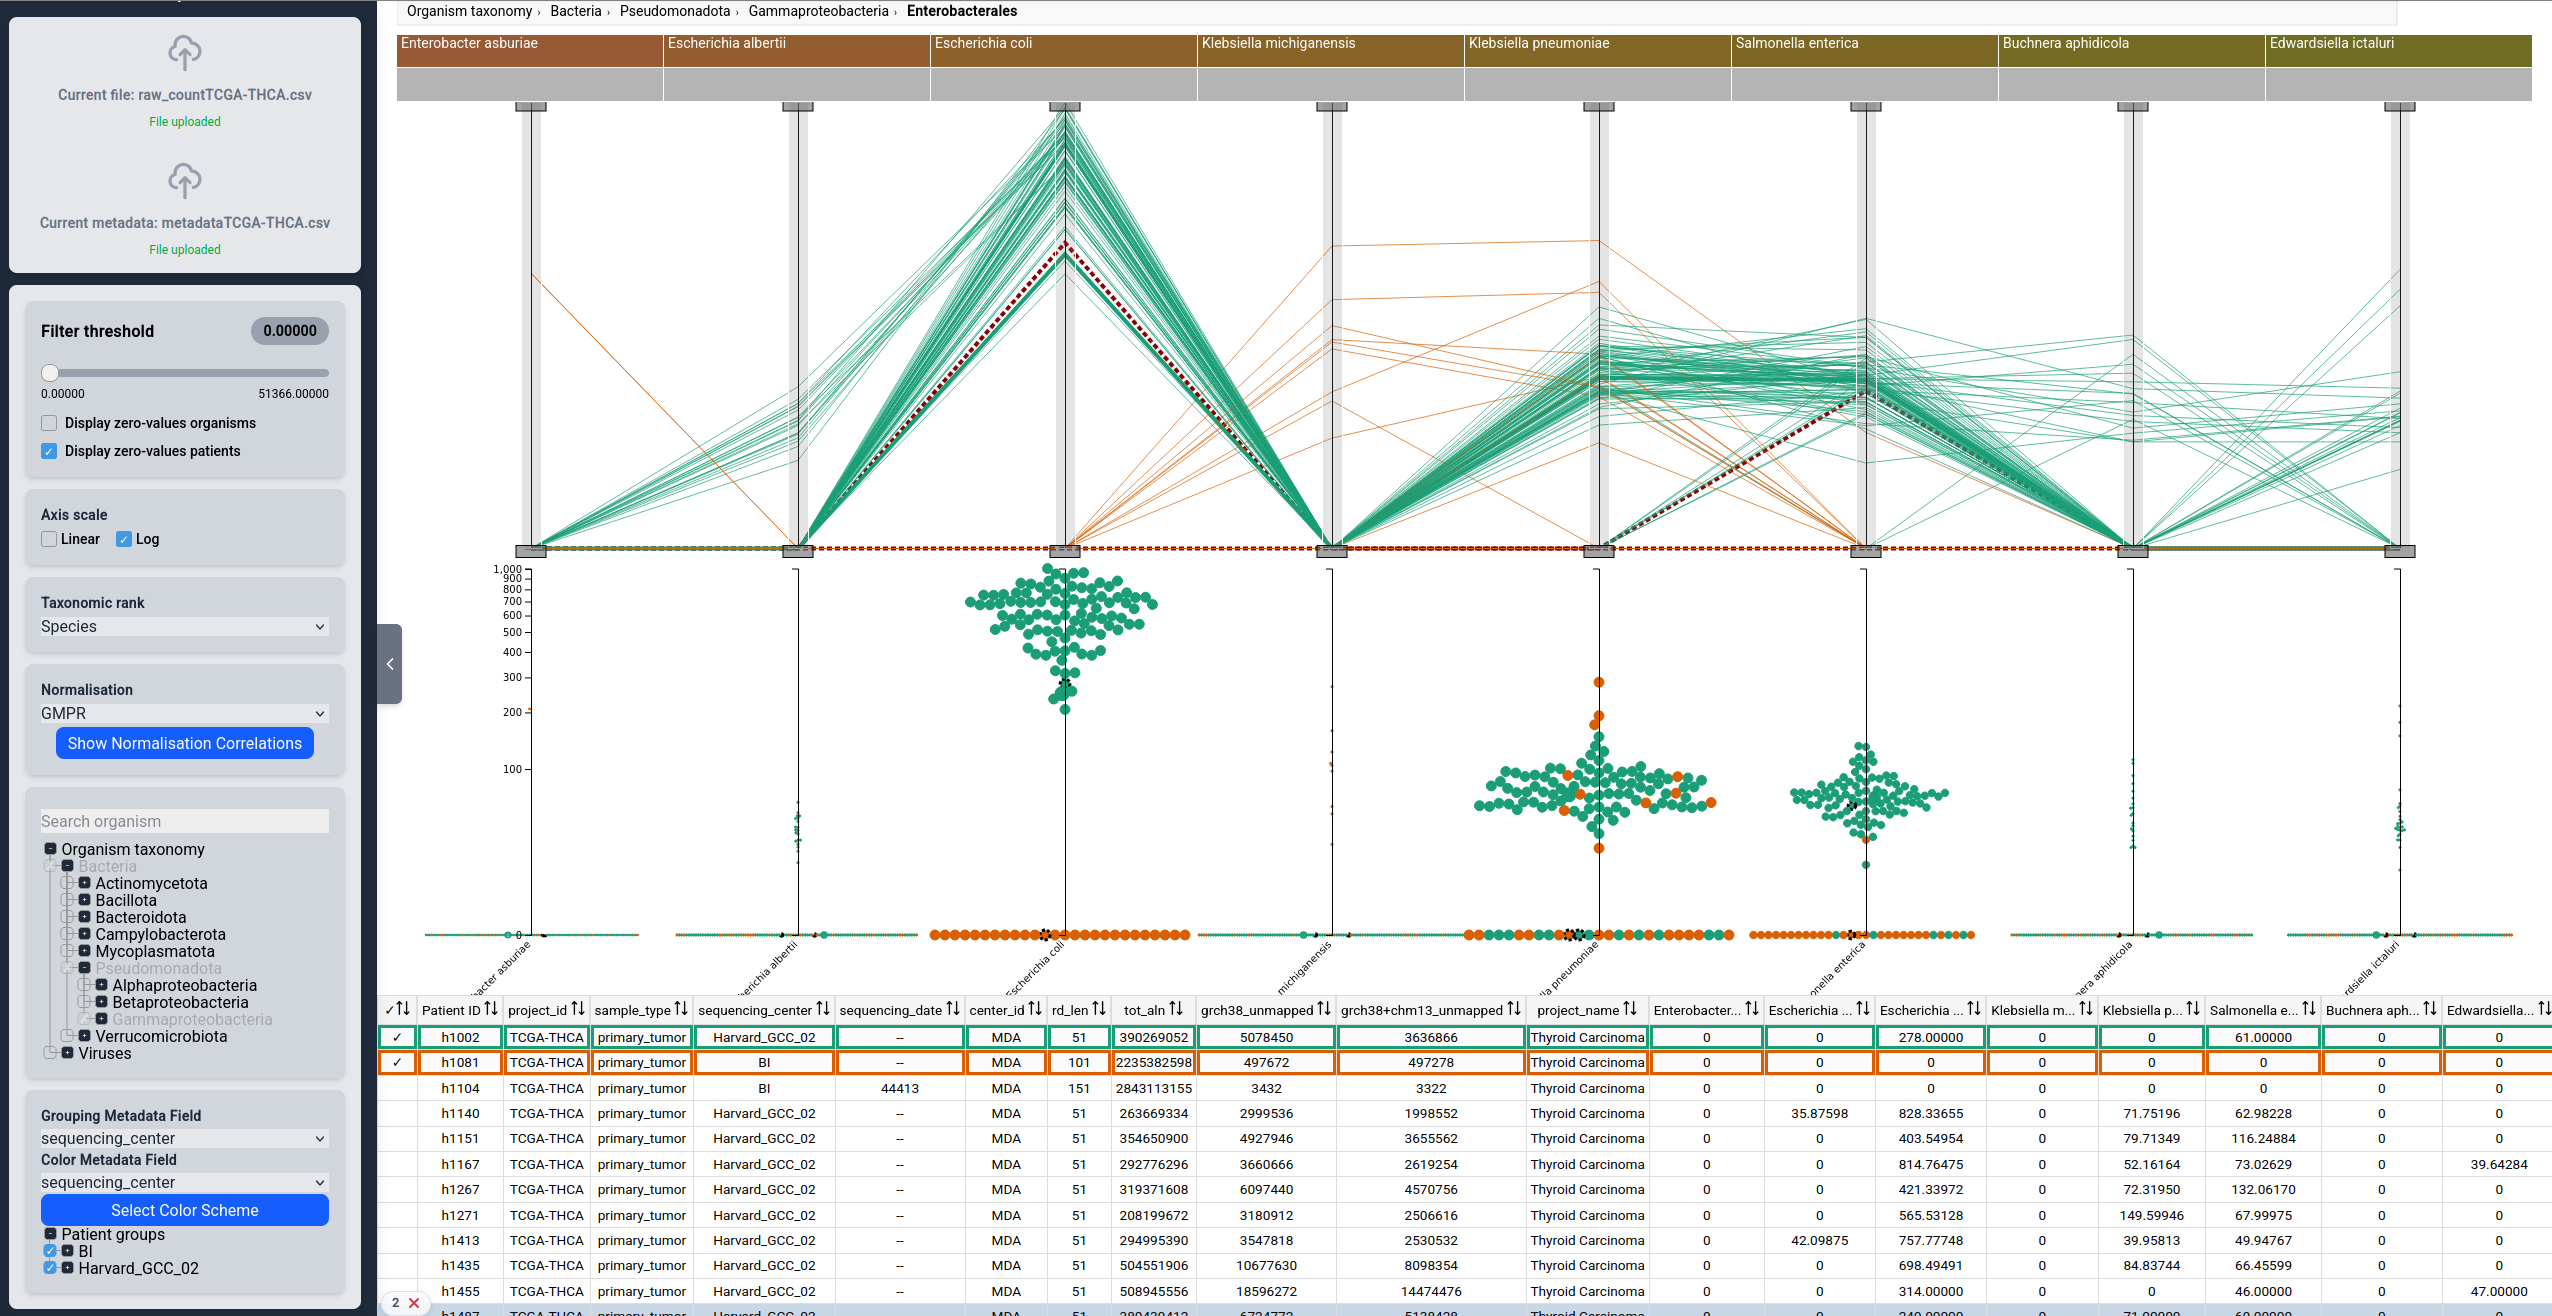
\includegraphics[width=\textwidth]{figures/supp3.png}
%    \caption{\textbf{Sample-level abundance profiles of Enterobacterales in TCGA-THCA.} TaxaLoom visualization restricted to species belonging to the order \textit{Enterobacterales} in the 98 TCGA-THCA \texttt{Primary Tumor} samples. Samples are coloured according to sequencing centre, allowing sequencing-associated abundance patterns to be identified across Enterobacterales species. Abundances were normalized using GMPR and displayed on a logarithmic scale.}
%    \label{figsupp:entero}
%\end{figure}

%\begin{figure}[htbp]
%    \centering
%    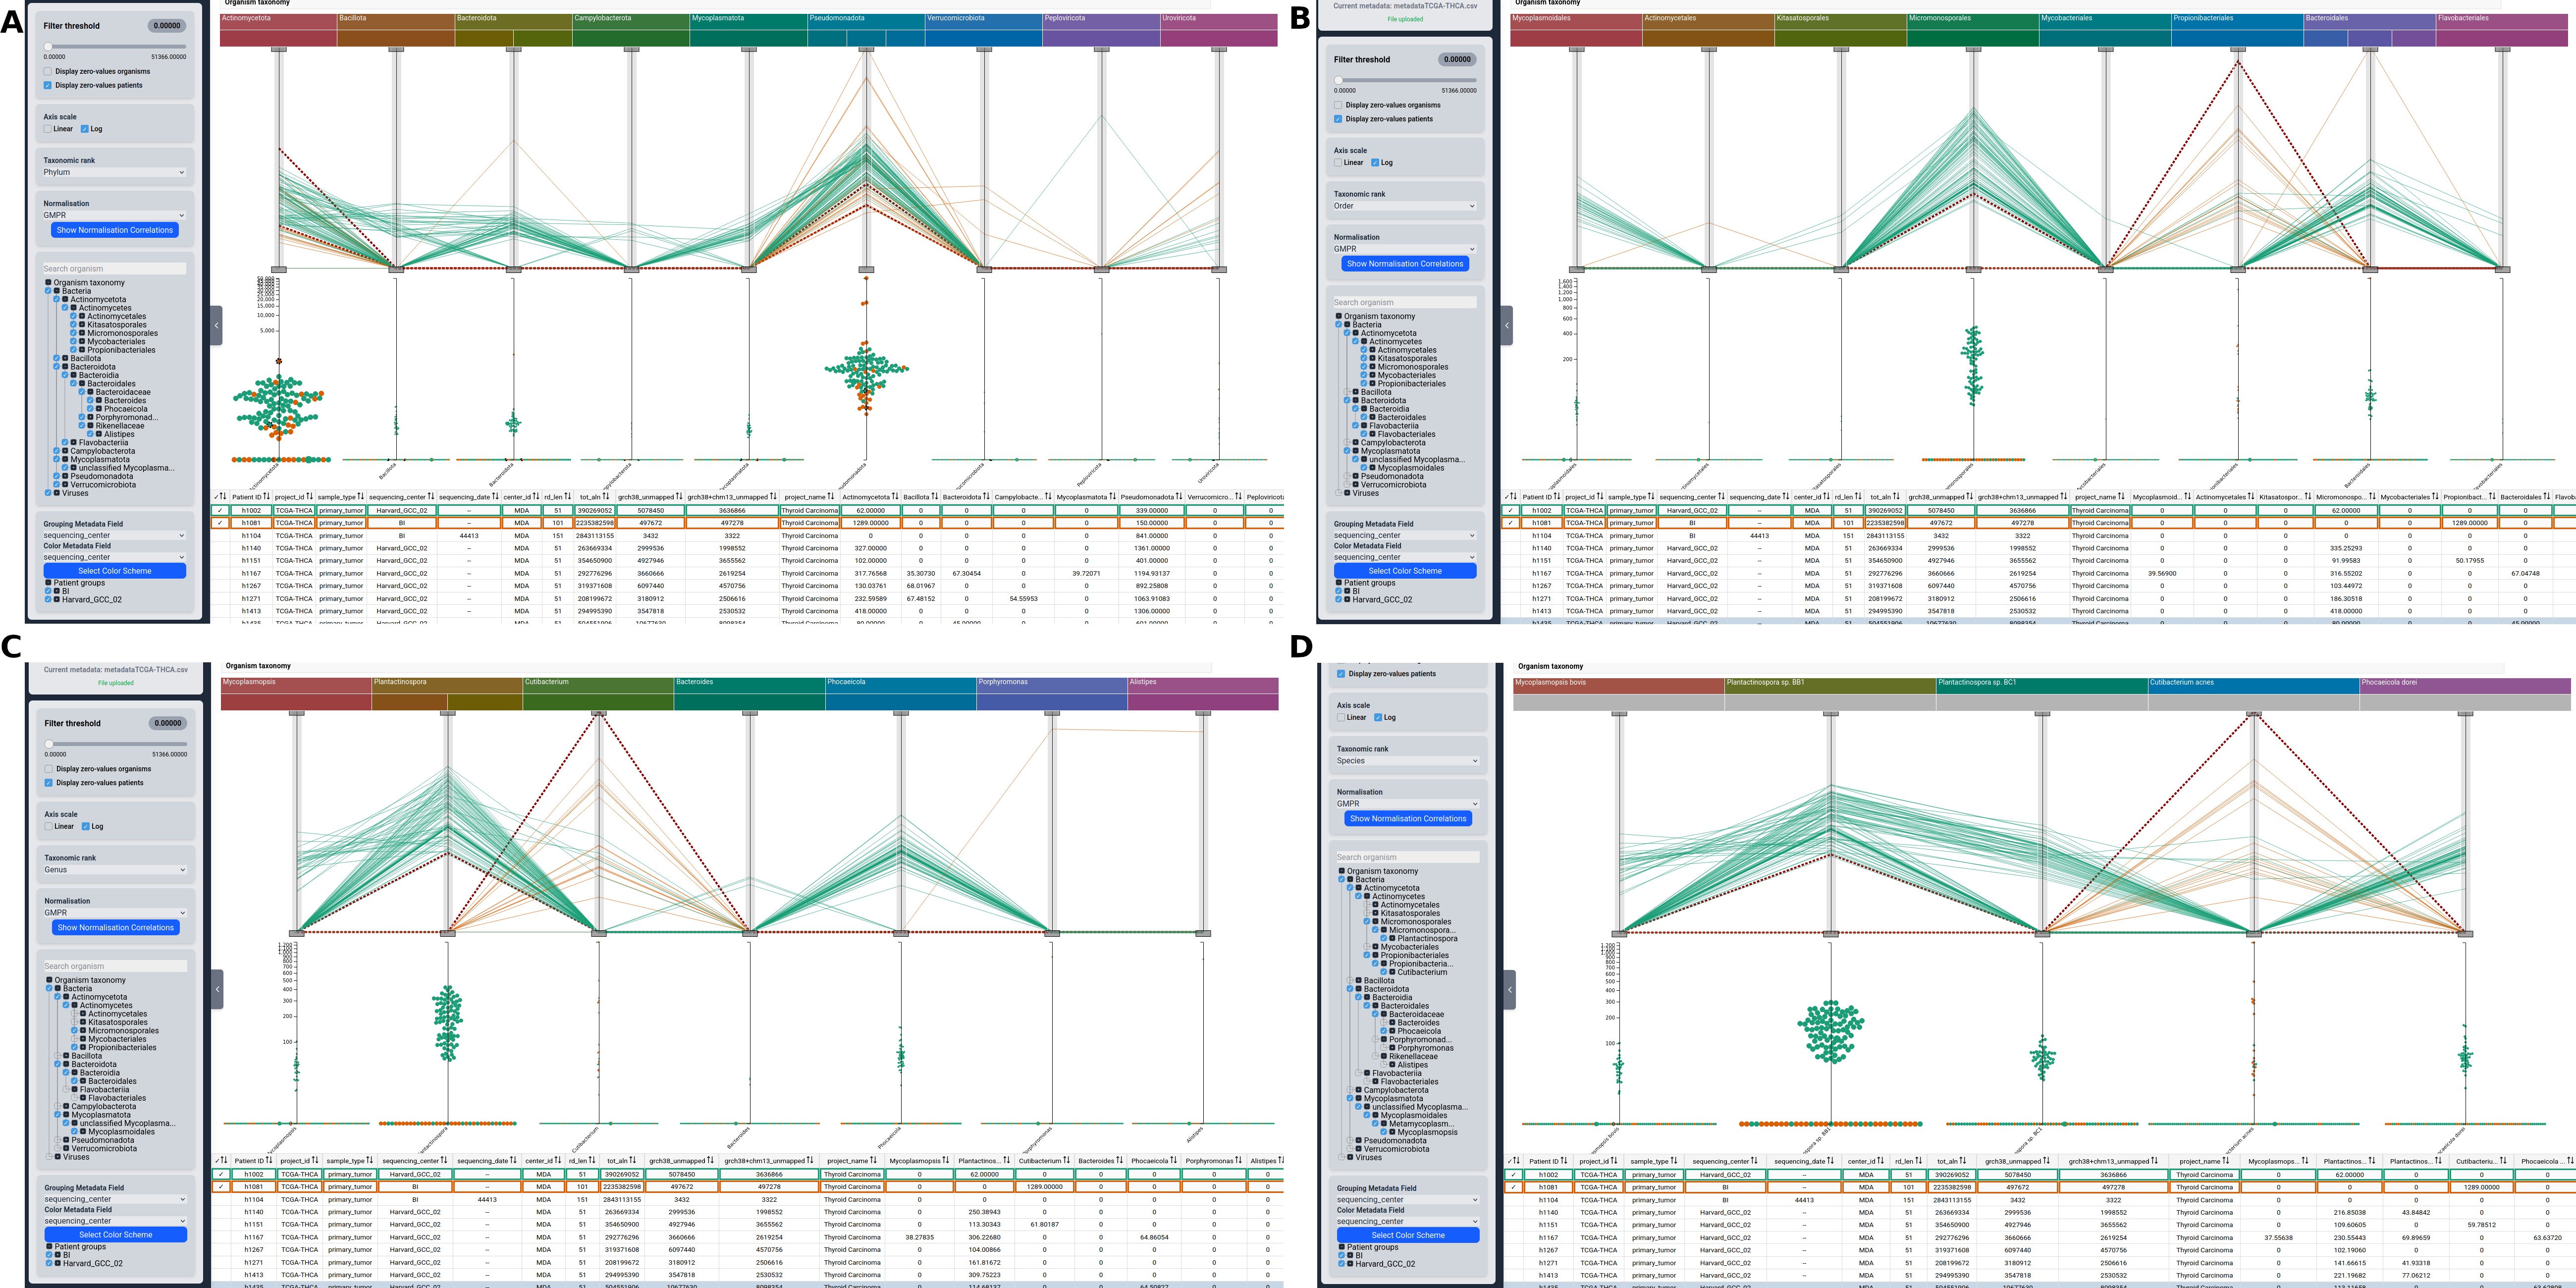
\includegraphics[width=\textwidth]{figures/supp2.png}
%    \caption{Progressive taxonomic filtering of TCGA-THCA microbial profiles using TaxaLoom. Taxonomic branches were successively filtered to focus on taxa exhibiting sequencing-associated abundance patterns. (\textbf{A}) Initial visualization at the phylum level. Selected phyla were removed to retain \textit{Actinomycetota}, \textit{Bacteroidota}, and \textit{Mycoplasmatota} for further exploration. (\textbf{B}) Resulting visualization at the order level, from which \textit{Mycoplasmoidales}, \textit{Micromonosporales}, \textit{Propionibacteriales}, and \textit{Bacteroidales} were retained. (\textbf{C}) Genus-level visualization, further restricted to \textit{Mycoplasmopsis}, \textit{Plantactinospora}, \textit{Cutibacterium}, and \textit{Phocaeicola}. (\textbf{D}) Final species-level visualization resulting from the successive taxonomic filtering. Abundances were normalized using GMPR and displayed on a logarithmic scale.}

%    \label{figsupp:conta_global}
%\end{figure}



\clearpage

\section{Supplementary Notes}

\subsection{Preprocessing methods available in TaxaLoom}\label{secA1}


Throughout this section, $y_{ji}$ and $q_{ji}$ denotes, respectively the raw and relative abundance of feature $i$ in sample $j$, and $N_j=\sum_{i=1}^{p}y_{ji}$ denotes the corresponding library size, where $p$ is the total number of features.

\subsubsection*{Binarisation}

Binarisation converts count data into presence-absence values by removing abundance information. Let $y_{ji}$ denote the raw count of feature $i$ in sample $j$.

The transformation is defined as

\[
x_{ji} =
\begin{cases}
1 & y_{ji} > 0 \\
0 & y_{ji} = 0
\end{cases}
\]

This transformation encodes only whether a feature is detected in a sample, disregarding quantitative abundance information.


\subsubsection*{Total Sum Scaling (TSS)}



Total sum scaling (TSS) transforms raw counts into relative abundances by normalizing each sample by its sequencing depth. Let $y_{ji}$ denote the raw count of feature $i$ in sample $j$.

The relative abundance is defined as

\[
q_{ji}=\frac{y_{ji}}{N_j}.
\]

which rescales each sample to sum to 1.


\subsubsection*{log2CPM}

log2 counts per million (log2CPM) rescales counts by library size and applies a $log_{2}$ transformation to stabilize the variance. Let $y_{ji}$ denote the raw count of feature $i$ in sample $j$.

The transformation is defined as

\[
x_{ji}=\log_2\left(\frac{y_{ji}+1}{N_j}\times10^6\right).
\]

where a pseudocount is added to avoid zeros before applying the log transform. It expresses counts as log-scaled counts per million reads, accounting for sequencing depth differences between samples.


\subsubsection*{TMM Normalisation}

TMM (Trimmed Mean of M-values) estimates a sample-specific scaling factor by comparing each sample to a reference sample \citep{robinson_scaling_2010}.

In the edgeR implementation, the reference sample $r$ is defined as the sample whose count-per-million upper quartile is closest to the mean upper quartile \citep{robinson_edger_2010}. For each feature $i$, an M-value representing the log-fold change between sample $j$ and the reference sample is computed as:

\[
M_{ji}=\log_{2}\left(\frac{y_{ji}/N_j}{y_{ri}/N_r}\right)
\]

where $y_{ji}$ and $y_{ri}$ denote the raw counts for feature $i$ in sample $j$ and reference sample $r$, respectively, and $N_j=\sum_i y_{ji}$ and $N_r=\sum_i y_{ri}$ are the corresponding library sizes.

An average abundance measure is also calculated as:
\[
A_{ji}=\frac{1}{2}\log_{2}\left(\frac{y_{ji}}{N_j}\cdot\frac{y_{ri}}{N_r}\right)
\]

The M- and A-values are then used to remove features with extreme fold changes or abundance values. Following the default TMM procedure, the 30\% highest and lowest M-values and the 5\% highest and lowest A-values are excluded \cite{robinson_scaling_2010}. The scaling factor is therefore estimated from features that are neither extreme in fold change nor in abundance.

The weight for feature $i$ and sample $j$ is defined as:

\[
w_{ji} = \frac{N_j - y_{ji}}{N_j \cdot y_{ji}} + \frac{N_r - y_{ri}}{N_r \cdot y_{ri}}
\]
The TMM scaling factor for sample $j$ relative to the reference is then obtained from the weighted mean of the M-values retained after trimming:

\[
\log_2(s_j)=\frac{\sum_{i \in \mathcal{I}} w_{ji} M_{ji}}{\sum_{i \in \mathcal{I}} w_{ji}},
\]

where $\mathcal{I}$ denotes the set of features retained after M- and A-value trimming. The resulting normalization factors $s_j$ are rescaled so that their product across samples equals one \citep{robinson_edger_2010}. As for RLE normalization, the effective library size is then obtained as:

\[
N_j^{*}=N_j s_j,
\]

where $N_j$ is the original library size of sample $j$.



\subsubsection*{RLE normalisation}

Relative log expression (RLE) normalization estimates sample-specific scaling factors using the median-ratio method proposed in \citep{anders_differential_2010}. For each feature $i$, the geometric mean of its counts across all $n$ samples is calculated:

$$
g_i=\left(\prod_{j=1}^{n}y_{ji}\right)^{1/n},
$$

where $y_{ji}$ denotes the raw count for feature $i$ in sample $j$. The resulting values $g_i$ define a reference abundance profile against which each sample is compared. The scaling factor $s_j$ for each sample is then calculated as the median of the ratios between its feature counts and the corresponding reference values:

$$
f_j={\operatorname{median}}\left(\frac{y_{ji}}{g_i}\right).
$$

In the edgeR implementation, these factors are rescaled so that their product across samples equals one \citep{robinson_edger_2010}. The resulting normalization factor $s_j$ is used to calculate the effective library size of sample $j$:

$$
N_j^{*}=N_j s_j,
$$

where $N_j$ is the original library size of sample $j$.





\subsubsection*{Blom transform}


The Blom transformation converts abundance values into rank-based normal scores \cite{blom_statistical_1958}. For each feature $i$, abundance values are first ranked across the $n$ samples. The rank $r_{ji}$ of feature $i$ in sample $j$ is then converted into a value between 0 and 1:


\[
q_{ji}=\frac{r_{ji}-3/8}{n+1/4},
\]
where $n$ is the number of samples. The resulting value $q_{ji}$ is then mapped to the corresponding quantile of the standard normal distribution using its inverse cumulative distribution function:

\[
x_{ji}=\Phi^{-1}(q_{ji}),
\]

where $\Phi^{-1}(\cdot)$ denotes the inverse cumulative distribution function of a normal distribution with mean 0 and standard deviation 1. The resulting $x_{ji}$ values are therefore rank-based normal scores that approximate a standard normal distribution while preserving the ordering of the original abundance values.


\subsubsection*{NPN transform}

The non-paranormal (NPN) transformation uses a rank-based Gaussianization procedure \citep{liu_nonparanormal_2009}. For each feature $i$, abundance values are ranked across the $n$ samples. The rank $r_{ji}$ of feature $i$ in sample $j$ is first mapped to a value between 0 and 1:

\[
q_{ji} = \frac{r_{ji}}{n+1},
\]

where $n$ is the number of samples.

These values are then transformed using the inverse cumulative distribution function of the standard normal distribution:

\[
x_{ji} = \Phi^{-1}(q_{ji}),
\]

yielding rank-based values that approximately follow a normal distribution.

In practice, a truncated version of the NPN transformation was used, as implemented in the \textit{huge} R package \citep{zhao_huge_2012}. Before applying the inverse normal transformation, values at the lower and upper extremes are constrained to predefined limits. This truncation prevents extreme ranks from producing excessively large positive or negative transformed values.

\subsubsection*{GMPR transform}

GMPR (Geometric Mean of Pairwise Ratios), as implemented in the \textit{MicrobiomeStat} R package, is a size-factor-based normalization method designed for sparse count data \cite{chen_gmpr_2018}.

For each pair of samples $(j,k)$, abundance ratios are calculated using only features that are non-zero in both samples. A pairwise ratio is defined as the median of these ratios:
\[
r_{jk} = \operatorname{median}_{i \in \mathcal{I}_{jk}} \left( \frac{y_{ji}}{y_{ki}} \right),
\]
where $\mathcal{I}_{jk} = \{i:y_{ji}>0,\;y_{ki}>0\}$ denotes the set of shared non-zero features between samples $j$ and $k$.

For each sample $j$, a sample-specific scaling factor $s_j$ is then calculated as the geometric mean of its pairwise ratios with the other samples:
\[
s_j = \left( \prod_{k \neq j} r_{jk} \right)^{\frac{1}{n}},
\]


where $n$ is the number of samples. The resulting scaling factor summarizes the abundance of sample $j$ relative to the other samples while reducing the influence of zeros by considering only features detected in both samples.

Normalized abundances are then obtained by dividing the raw counts by the corresponding scaling factor:

\[
x_{ji} = \frac{y_{ji}}{s_j}.
\]

\subsubsection*{CSS transform}

Cumulative sum scaling (CSS), implemented in the \textit{metagenomeSeq} R package, is a normalization method designed for sparse microbiome count data \citep{paulson_differential_2013}.

CSS determines a percentile of the count distribution from the data, above which highly abundant features are excluded from the calculation of the scaling factor. For each sample $j$, the scaling factor $s_j$ is then calculated as the cumulative sum of counts up to the selected percentile:

$$
s_j=\sum_{i:\,y_{ji}\le q_{\hat l}(y_j)}y_{ji},
$$

where $q_{\hat l}(y_j)$ denotes the count value corresponding to the selected percentile in sample $j$.

Normalized abundances are obtained by dividing each raw count by the corresponding scaling factor:

$$
x_{ji}=\frac{y_{ji}}{s_j}.
$$

By calculating the scaling factor without the most highly abundant features, CSS reduces their influence on the normalization.


\subsubsection*{AsinSquareRoot}

The arcsine square-root transformation is applied to relative abundance data to stabilize variance, particularly for proportions close to 0 or 1. Let $q_{ji}$ denote the relative abundance of feature $i$ in sample $j$, obtained after total sum scaling.

The transformation is defined as

\[
x_{ji} = \arcsin\left(\sqrt{q_{ji}}\right),
\]

The transformation reduces the dependence of the variance on the mean that is characteristic of proportional data, producing values with a more stable variance across the range of relative abundances.

\subsubsection*{CLR transform}

The centered log-ratio (CLR) transformation maps relative abundances to a log-ratio scale relative to the geometric mean of all features within a sample \citep{aitchison_statistical_1982}. Let $g_j$ denote the geometric mean of the relative abundances in sample $j$.

The transformation is defined as:

\[
x_{ji} = \ln\left(\frac{q_{ji}}{g_j}\right),
\]

where

\[
g_j = \left(\prod_{k=1}^{p} q_{jk}\right)^{1/p},
\]

and $p$ is the total number of features. The resulting values express the abundance of each feature relative to the geometric mean abundance of all features within the same sample.

\subsubsection*{rCLR transform}

The robust centered log-ratio (rCLR) transformation is a modification of the CLR transformation that accommodates zero values by calculating the geometric mean using only non-zero features \citep{martino_novel_2019}.

For each sample $j$, the geometric mean is calculated using only non-zero relative abundances:

\[
g_j=\exp\left(\frac{1}{m_j^{+}}\sum_{k:q_{jk}>0}\ln(q_{jk})\right),
\]

where $m_j^{+}$ denotes the number of non-zero features in sample $j$.

The rCLR transformation is then defined as:

\[
x_{ji}=
\begin{cases}
\ln\left(\frac{q_{ji}}{g_j}\right) & q_{ji}>0,\\
0 & q_{ji}=0.
\end{cases}
\]

The resulting values express each non-zero feature as a log-ratio relative to the geometric mean of the non-zero features within the same sample, while zero values remain zero in the transformed data.


\subsection{Microbial abundance filtering}\label{secA2}

Both datasets used in the case studies were derived from host-dominated sequencing data and we therefore add an additional filtering step before their use in TaxaLoom. The Cleveland cohort was generated from total-RNA sequencing of blood samples, in which human-derived reads represented the majority of the sequencing data \cite{nganou-makamdop_translocated_2021,colajanni_benchmarking_2026}. Similarly, the TCGA microbial profiles were obtained from the reanalysis of human whole-genome sequencing (WGS) data \citep{ge_comprehensive_2025}. As the microbial signal represents only a small fraction of these datasets, we applied dataset-specific filtering procedures to reduce low-abundance and potentially spurious taxonomic classifications before visualization. 

We used a similar strategy for both dataset as they were reanalysed using similar procedure. 

\subsubsection*{Cleveland cohort filtering} \label{secA3}

The Cleveland cohort, originally described by \citet{lederman_immunologic_2011} and subsequently sequenced and analysed by \citet{nganou-makamdop_translocated_2021}, comprised 55 HIV-infected individuals receiving combined antiretroviral therapy (cART). Participants were classified as immune responders ($n=11$) or immune non-responders ($n=44$) based on CD4+ T-cell counts above 500 or below 350 cells/$\mu$L, respectively, after at least 24 months of virologic suppression on cART \citep{lederman_immunologic_2011}. Individual CD4+ T-cell counts were also available, providing both categorical immune response status and a quantitative measure of immune recovery.

Raw sequencing data were retrieved from the Sequence Read Archive (SRA) and reanalysed as described in our previous benchmarking study \citep{colajanni_benchmarking_2026}. The resulting genus-level raw count data were retrieved from this study, while the associated clinical metadata were obtained from \citet{nganou-makamdop_translocated_2021}.

CD4+ T-cell counts were log-transformed to facilitate visualization.

Following taxonomic classification, genera considered biologically implausible in human blood were manually excluded based on their known host range and ecology. This filtering removed 23 genera, including plant-associated viruses and pathogens: \textit{Orthotospovirus} \citep{kormelink_bunyavirales_2021}, \textit{Albugo} \citep{kemen_gene_2011}, \textit{Phytophthora} \citep{meng_phytophthora_2014}, \textit{Entyloma} \citep{kruse_broad_2018}, \textit{Sporisorium} \citep{zhao_sporisorium_2022}, \textit{Stenocarpella} \citep{health_plh_pest_2022}, \textit{Sclerotinia} \citep{derbyshire_evolutionary_2022}, \textit{Taphrina} \citep{nigon_exploring_2026}, and \textit{Zymoseptoria} \citep{quaedvlieg_zymoseptoria_2011}. Genera associated with highly specific non-human or environmental niches were also removed, including the bee gut symbiont \textit{Gilliamella} \citep{kwong_evolution_2015}; the haloarchaea \textit{Halobacterium} and \textit{Haloplanus} \citep{fendrihan_extremely_2006}, \textit{Halorubrum} and \textit{Natronomonas} \citep{kamekura_diversity_1998}, and \textit{Natrinema} \citep{strakova_natrinema_2023}; the wood- or tree-associated fungi \textit{Hornodermoporus} \citep{yuan_species_2023}, \textit{Chrysoporthe} \citep{van_der_nest_ima_2021}, \textit{Immersiporthe} \citep{chen_serious_2013}, and \textit{Phlebiopsis} \citep{iwata_omics_2021}; the mushroom-forming genus \textit{Entoloma} \citep{liu_additions_2025}; the insect-parasitic nematode \textit{Hexamermis} \citep{poinar_hexamermis_1985,lee_hexamermis_2026}; and the dung-associated fungus \textit{Sordaria} \citep{newcombe_revisiting_2016}. Finally, \textit{Sinsheimervirus} was excluded because this genus contains PhiX174, which is commonly used as an Illumina sequencing control \citep{illumina_phix_control}. 

To reduce low-abundance taxonomic assignments, read-count cutoffs ranging from 1 to 50 reads were evaluated independently for each sample. For each cutoff, taxa with fewer reads were considered absent and their counts were set to zero. The resulting relationship between the minimum abundance required for detection and the number of taxa remaining in each sample is shown in Figure~\ref{figsuppsupp}.

A sample-specific cutoff was selected as the first point at which the mean relative decrease in the number of taxa reached 5\% over a sliding window of five consecutive values. This criterion was designed to identify the beginning of a plateau, beyond which increasing the cutoff produced relatively little change in the number of detected taxa, thereby limiting low-abundance classifications potentially resulting from spurious taxonomic assignments.

\begin{figure}[htbp]
\centering
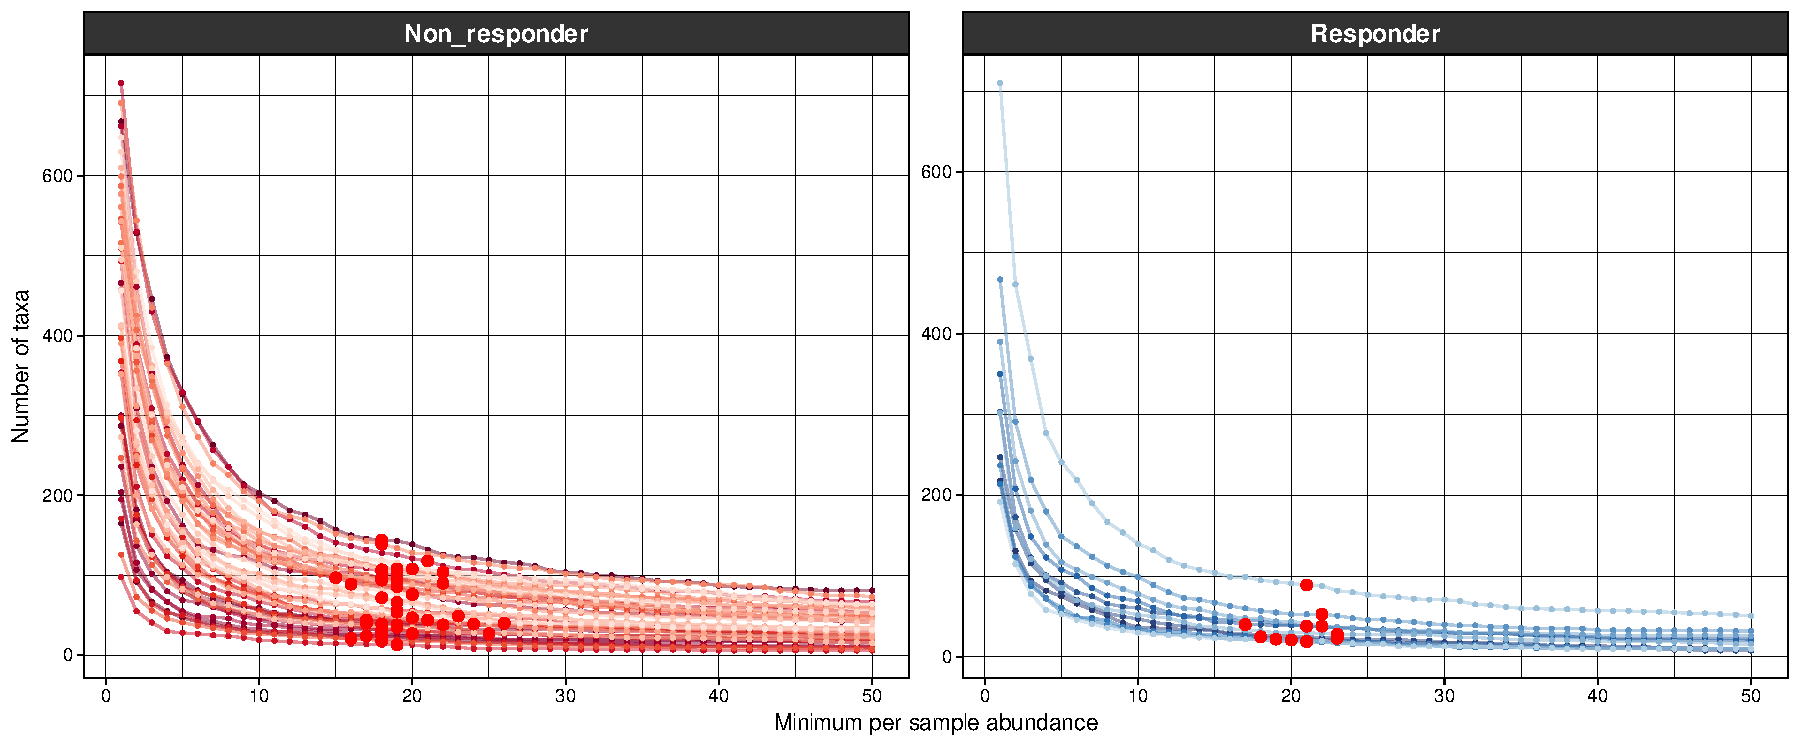
\includegraphics[width=\textwidth]{figures/supp_fig_filtration_cleveland.pdf}
\caption{Sample-specific abundance filtering for the Cleveland cohort. Number of taxa retained in each sample as a function of the minimum read-count threshold required to consider a taxon present. Taxa with counts below the corresponding threshold were considered absent and their counts were set to zero. Red points indicate the threshold selected independently for each sample, defined as the first point at which the mean relative decrease in the number of retained taxa reached 5\% over a sliding window of five consecutive thresholds.}
\label{figsuppsupp}
\end{figure}

For the case application, we focused on the 29 bacterial genera previously reported as differentially abundant between immune responders and immune non-responders by \citet{nganou-makamdop_translocated_2021}: \textit{Mycobacterium}, \textit{Kocuria}, \textit{Microbacterium}, \textit{Lactococcus}, \textit{Hymenobacter}, \textit{Sphingobacterium}, \textit{Xanthomonas}, \textit{Serratia}, \textit{Klebsiella}, \textit{Achromobacter}, \textit{Comamonas}, \textit{Hydrogenophaga}, \textit{Acidovorax}, \textit{Variovorax}, \textit{Ramlibacter}, \textit{Delftia}, \textit{Roseateles}, \textit{Rhizobacter}, \textit{Rubrivivax}, \textit{Massilia}, \textit{Burkholderia}, \textit{Ralstonia}, \textit{Methylophilus}, \textit{Sphingobium}, \textit{Novosphingobium}, \textit{Ochrobactrum}, \textit{Methylobacterium}, \textit{Brevundimonas}, and \textit{Rickettsia}.

Prior to visualization, genera detected in fewer than 22 of the 55 samples (40\% prevalence) were excluded to reduce sparsity. The remaining abundance counts were normalized using the trimmed mean of M-values (TMM) method. Within TaxaLoom, genera were further filtered using the built-in Wilcoxon rank-sum test, retaining those with a nominal $p<0.05$. This resulted in 9 genera selected for visualization: \textit{Lactococcus}, \textit{Serratia}, \textit{Klebsiella}, \textit{Comamonas}, \textit{Variovorax}, \textit{Delftia}, \textit{Massilia}, \textit{Sphingobium}, and \textit{Methylobacterium}.


\subsubsection*{TCGA-THCA filtering} \label{secA4}

Reanalysed TCGA microbial abundance data and associated metadata were obtained from \citet{ge_comprehensive_2025}. The complete dataset comprised 5,734 whole-genome sequencing samples and 11,389 detected species. Complete taxonomic lineages were reconstructed from the taxonomic identifiers provided in the dataset using TaxonKit \citep{shen_taxonkit_2021}. Samples with fewer than 1,000 total microbial counts were excluded to ensure sufficient microbial signal for subsequent exploration.

For the technical case application, the analysis was restricted to TCGA thyroid carcinoma (TCGA-THCA). The complete TCGA dataset was too large for practical interactive exploration with TaxaLoom, while the objective of this case application was to investigate technical covariates rather than cancer-specific abundance patterns. TCGA-THCA was selected because it contained a large number of \texttt{Primary Tumor} samples from both sequencing centres while remaining sufficiently small for efficient exploration. The resulting dataset comprised 122 \texttt{Primary Tumor} samples, including 26 from \texttt{BI} and 96 from \texttt{Harvard\_GCC\_02}.

To further reduce low-abundance taxonomic assignments within the retained samples, sample-specific abundance cutoffs ranging from 1 to 250 counts were evaluated independently for each sample. For each cutoff, species with counts below the threshold were considered absent and their counts were set to zero. The selected cutoff corresponded to the first point at which the mean relative decrease in the number of retained taxa fell below 1\% over a sliding window of five consecutive cutoff values (Figure~\ref{figsuppsupp2}). The wider range of candidate cutoffs and more stringent plateau criterion compared with the Cleveland cohort were used to accommodate the greater heterogeneity in microbial abundance observed across the TCGA samples.


\begin{figure}[htbp]
\centering
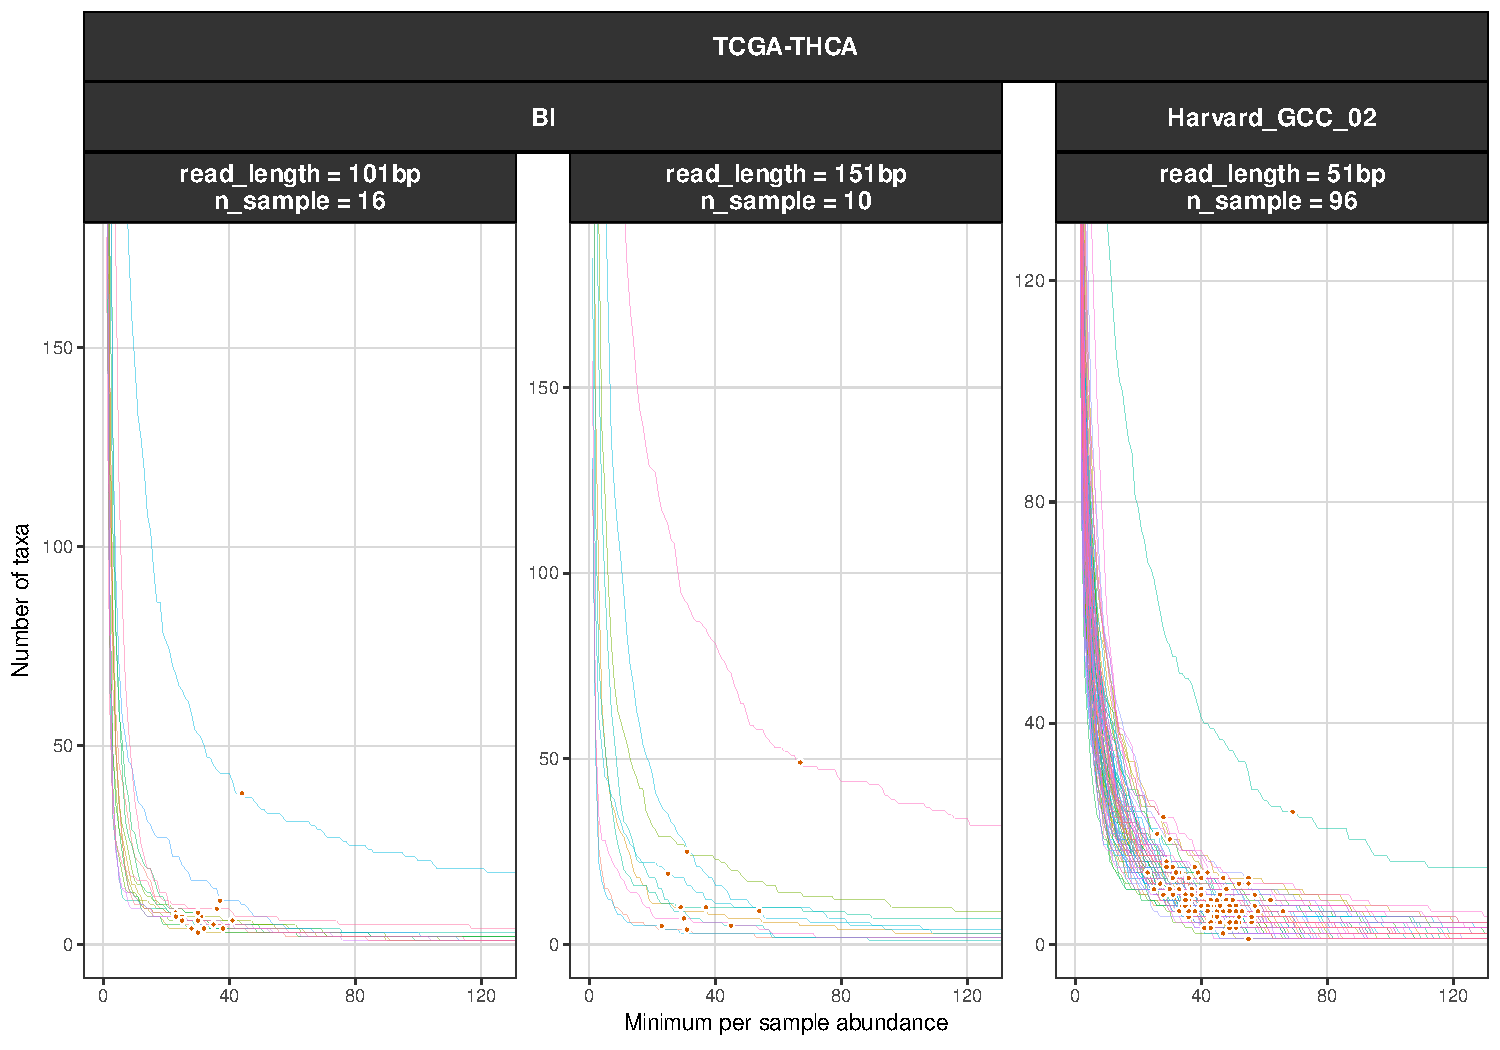
\includegraphics[width=\textwidth]{figures/supp_filtration_THCA.pdf}
\caption{Sample-specific abundance filtering for the TCGA-THCA, primary tumor samples. Number of taxa retained in each sample as a function of the minimum read-count threshold required to consider a taxon present. Taxa with counts below the corresponding threshold were considered absent and their counts were set to zero. Red points indicate the threshold selected independently for each sample, defined as the first point at which the mean relative decrease in the number of retained taxa reached 1\% over a sliding window of five consecutive thresholds.}
\label{figsuppsupp2}
\end{figure}


\newpage


\putbib[sn-bibliography]

\end{appendices}




\end{bibunit}




\end{document}
